\documentclass{book}
\usepackage{amsmath}
\usepackage[acronym]{glossaries}
\usepackage[backend=biber, natbib=true]{biblatex}
\usepackage{tikz}
\usetikzlibrary{arrows,positioning,shapes.geometric, calc}
\usepackage{amsthm}
\usepackage{graphicx}
\usepackage{caption}
\usepackage{subcaption}
\usepackage{booktabs}
\newtheorem{mydef}{Definition}
\usetikzlibrary{positioning}
\usepackage{adjustbox}
\usepackage{lscape}
\usepackage{setspace}
\linespread{1.5}

\bibliography{/home/robert/Documents/library.bib}
\title{The Genetics of Aggressive Behavior}
\author{Robert Milan Porsch}
\date{\today}
% Evo history
\newacronym{rhp}{RHP}{Resource Holding Power}
\newacronym{rv}{RV}{Resource Value}
\newacronym{adhd}{ADHD}{Attention Deficit Hyperactivity Disorder}
\newacronym{sst}{SST}{Sexual Selection Theory}
\newacronym{vntr}{VNTR}{Variable Number Tandem Repeat}


% Methods twins
\newacronym{sem}{SEM}{Structural Equation Model}
\newacronym{mz}{MZ}{monozygotic}
\newacronym{dz}{DZ}{dizygotic}

% Methods gwas
\newacronym{gwas}{GWAS}{Genome Wide Association Study}
\newacronym{snp}{SNP}{Single Nucleotide Polymorphism}
\newacronym{ld}{LD}{Linkage Disequilirium}
\newacronym{pca}{PCA}{Principle Component Analysis}
\newacronym{pc}{PC}{Principle Component}
\newacronym{fdr}{FDR}{False Discovery Rate}
\newacronym{gcta}{GCTA}{Genome-wide Complex Trait Analysis}
\newacronym{maf}{MAF}{Minor Allele Frequency}
\newacronym{skat}{SKAT}{sequence kernel association test}

%\tikzexternalize % for faster compilation

\begin{document}
\maketitle
\chapter{Introduction}
\label{cha:introduction}

% dramatic entry
Aggressive behavior has potential beneficial and harmful consequences for the aggressor.
While aggression caries a serious risk of bodily harm for the aggressor, it also has the potential to increase access to resources and higher social status.
The nature and cause of such behavior has always been of interest to social and biological focused researchers and much scientific effort has been spend to investigate the various different facets of this complex behavior.
While previous research has been focused on environmental as well as biological causes of aggressive behavior, here I will solely focus on potential biological mechanisms of human aggression.
Specifically I will investigate potential genetic causes of human aggressive behavior via a variety of different statistical methods.

The first chapter of this thesis will review the existing literature in regards to the definition and forms of aggression, as well as evolutionary theories and known genetic risk factors associated with this complex behavior.
Subsequently, I will give an overview of the statistical methods used within this thesis.
Chapter 3 describes my investigation of over 28,000 twin pairs to examine the longitudinal heritability of childhood aggression.
The next chapter describes the exploration of specific molecular genetic marker associated with risk taking and aggression in over 150,000 unrelated individuals.
Afterwards, in chapter 5, I will examine the genetic overlap of various traits with aggressive behavior.
Chapter 6 will outline a newly developed method to test for distributional differences of rare mutation between aggressive and non-aggressive subjects.
At last I will discuss my findings in details and outline future research directions.

\section{Definition of Aggression}
\label{sec:overview_of_reseach_in_aggression}

One can define human aggression as a behavior intended to cause physical or emotional harm to others~\cite{Anderson2002}.
However, this definition is rather incomplete.
It is also important to consider the unwilling participation of the victim as well.
Hence behaviors in which the target does not intend to avoid the aggressive behavior, such as in sexual masochism~\cite{Berkowitz1993,Baumeister1989,Baron2007,Geen2001} should not be considered an aggressive act.
Thus the motivation of the victim to avoid such harm plays an important role in the definition of aggression.  
Therefore I will use the following working definition:
\begin{mydef}[Aggression]\label{def:aggression}
	`Aggression is the delivery of an aversive stimulus form one person to another, with intent to harm and with an expectations of causing such harm, when the other person is motivated to escape or avoid the stimulus'~\cite{Geen2001}
\end{mydef}

While aggression is most commonly associated with physical harm, Definition~\ref{def:aggression} also includes a broader spectrum.
Non violent behavior, like spreading gossips, damaging a victims property either due to emotional anger or as a planned action to gain an advantage to a higher goal.
This large spectrum of aggression makes it necessary to specify the broader dimension of this behavior.

\subsection{Forms of aggression}
\label{sub:forms_of_aggression}

One can separate aggressive behavior into \textit{affective aggression} and \textit{instrumental aggression}.
While \textit{affective aggression} is characterised as emotional, impulsive, thoughtless and unplanned behavior, \textit{instrumental aggression} is defined as a planed and proactive behavior to obtain a certain higher goal~\cite{Berkowitz1993,Geen2001}.
This distinction has been extended by a number of similar concepts, such as \textit{reactive/proactive} and \textit{offensive/defensive} aggression.
While these terms have slightly different meaning, depending on situation and field of research, the general concept remains similar~\cite{Geen2001, Blanchard2005b}.
In psychology, for example, the term \textit{affective aggression} and \textit{instrumental aggresssion} has been established, but more recently authors have used the terms \textit{reactive} and \textit{proactive} aggression~\cite{Geen2001}.
Thus aggressive action in response to a provocation, such as self-defence and in anger, is \textit{reactive aggression} while planned, un-provoked aggression is called \textit{proactive}.

However, despite the differences in terminology it is important to emphasise the strong negative emotional state of \textit{affective/reactive} aggression.
This state, often described as \textit{anger}, launches and guides affective aggression  and is often caused by some form of provocation~\cite{Geen2001}.
Nevertheless, \citet{Frijda1994} suggested that \textit{affective/reactive aggression} is not necessary impulsive.
In some situations a delayed response between provocation and aggressive response is observed. 
In particular long term grudges, or \textit{hatreds} are preoccupations which go beyond the initial provocation but remain deeply emotional.
Thus I will use the term \textit{impulsive aggression} to refer to impulsive, emotional guided aggressive behavior.

In contrast \textit{Instrumental/proactive aggression} is characterised by the absence of an emotional strong cause to cause harm.
For example, the use of gossip and bad-mouthing of a colleague in order to obtain higher chances of receiving a promotion is done in a planned manner with the aim of a higher goal (receiving the promotion).
However, it is often difficult to distinguish actions into affective and instrumental aggression since both forms are not mutually exclusive.
\citet{Geen2001} gave the example of a mother who uses corporal punishment to modify her child's behavior, while still reacting in anger when observing the undesired child's behavior.
Hence mixing a planned aggressive act towards a higher goal with an emotional, angry state.

Both forms of aggression, affective and instrumental, can be either physical or verbal.
While physical aggression in humans is homologous to other animals, verbal aggression, also called \textit{indirect}, \textit{relational} and \textit{social} aggression, is relatively distinct to humans~\cite{Archer2005}.
These verbal behaviors cause harm to others by gossiping, spreading rumors, or excluding other from social groups.
While the terms \textit{indirect}, \textit{relational}, and \textit{social} aggression have been differently conceptualized in the past~\cite{Archer2001}, they are expressed in common behaviors and can be contrasted to physical, \textit{direct}, aggression.
Hence the terms are more similar than distinct and I will therefore proceed to call all them \textit{indirect} aggression in order to distinguish it more from the physical, more direct aggressive behavior~\cite{Archer2005}.

Research in animals have often used a slightly different terminology.
Investigations often have distinguished between \textit{offensive} and \textit{deffensive} aggression~\cite{Blanchard2005b}.
Similar to \textit{affective} aggression \textit{offensive} attacks arise from a response to a threat to the animals resources, thus are the response to a certain provocation.
These resources could be sexual partners, food, social status, or in the case of humans, also money.
On the other hand, \textit{deffensive} aggression is the result to a direct threat to the subject life, a concept closer related to \textit{instrumental} aggression.
While this distinction might hold in mice and rats, the separation between \textit{offensive} and \textit{deffensive} aggression is more blurred in primates, including humans.
For example, humans are known to hunt lions and other predators.
In contrast to non-predators, these animals are, for the most part, not eaten which would suggest a form of defensive aggressive behavior.
However, within most human cultures killing a large predator is seen to enlarge ones social status by showing strength and courage towards the others.
A behavior which could be described as an \textit{offensive} action.
Thus the distinction between \textit{offensive} and \textit{deffensive} aggression is blurred.
This blurred distinction reflects the above described example of the punishing mother by \citet{Geen2001}.
However, \citet{Blanchard2005b} suggest, while the separation between \textit{offensice/affective} a and \textit{defensive/instrumental} might be blurred in humans, the distinction holds in general.
The authors suggest that rather insufficient analysis and not a disconnection between animal and human behavior are responsible for the blurred distinction within humans.
However, \citet{Blanchard2005b} provide little evidence for their claims and one can argue that the complexity of human society makes a comparison between sub-categories of aggressive behavior across species especially difficult. 
Nevertheless, animal studies have provided valuable insight into aggressive behavior and I will outline a number of experimental findings in animal studies in later sections.

To conclude, one can distinguish between \textit{affective} and \textit{instrumental} forms of human aggression which can be expressed either \textit{direct} or \textit{indirect}.
Research in non-humans have often distinguish between \textit{offensive} and \textit{defensive} forms of aggression.
A distinguish which is more blurred in humans.
I will next consider evolutionary theories in regards to aggression in humans and animals alike.
I will show that aggressive behavior has a strong evolutionary background and that genes which regulate such behavior are under stabilizing selection.

\section{Evolutionary Theories}
\label{sec:evolutionary_theories}

Historically, research of aggression has been divided into nurture versus nature~\cite{Archer2009}. 
Proponents of the nurture side have argued that aggressive behavior is caused by environmental influences, while supports of the nature side of the discussion supported the idea that only differences in the genetic architecture are able to explain individual differences in aggressive behavior.
Today's view is less polarized and acknowledges that both, nature and nurture play a crucial part in aggression.
While not disregarding the environmental aspect of aggression I will mostly focus on the genetic and biological mechanisms of aggressive behavior.
In the following section I will outline evolutionary concepts helpful in explaining and understanding individual differences of aggression. 

Evidence for a long history of human aggression can be found in  palaeontological findings of broken bones, rips and smashed skulls, unexplainable without the consideration of weaponry force.
Occasional findings of weapon fragments in skeletal rib cages suggest that violence and aggression has been part of the human evolutionary history. 
\citet{Buss1997}, one of the founder of evolutionary psychology, suggested that all psychological mechanisms and behavior, including aggression, originate in the evolutionary principle of selection.  
These mechanisms are aimed to solve specific adaptive problems.
Hence some variants of those behaviors and psychological mechanisms might solve certain problems better than others, thus improving overall fitness.
This results in the preservation, replication and spreading of theses variants through a population~\cite{Buss1997}.

\citet{Buss1997} suggested \textit{seven} adaptive problems to which aggressive behavior might be an evolutionary solution.
For example \textit{Co-Opt the Resources of Others}, which can be defined as the use of physical or psychological force to obtain resources hold by another individual or group, can give the aggressors significant advantages in terms of survival and reproduction.
These resources could mean food, water, land or sexual partners.
An example of this can be seen in aggressive behavior of children.
\citet{Campbell1995} noted that aggression among toddlers is often about resources, such as toys, suggesting that this behavioral adaptations is an deeply rooted evolutionary strategy.

Aggression can also be useful in \textit{defending against an attack}.
Since attacking aggressors are a serious threat to valuable resources.
Aggression can be an effective strategy in defending against individuals or groups.
Further, it can be also an adaptive strategy to foster a reputation that would deter potential aggressors~\cite{Buss1997}.
Thus avoiding the potential cost of a physical conflict while defending one's resources.

Another evolutionary benefit of aggression can be found in the social hierarchies in groups.
For example, men who win fights and defeat opponents gain power and status in many societies~\cite{Hill1996}.
The gain in social status can be beneficial in accessing resources and mates~\cite{Archer2009}.
Indeed, hierarchical order in social groups is often established by means of aggressive behavior which enables high ranked individuals priory access to food and patterns~\cite{Lindenfors2011}. 
However, aggression can also result in an decline in status.
\citet{Buss1997} suggested for example that a physical conflict between two professors in a faculty meeting would result in an decline in reputation.
Thus display of aggression is not acceptable in all social situations or helpful in achieving a goal.

In the context of reproduction one should consider aggression towards the same-sex separate of male-female aggression.
Aggression towards same-sex individuals is sometimes aimed to reduce their social status and therefore make them less attractive to the other sex~\cite{Buss1990}.
Hence inflicting damage on a rival directly translates to an increased benefit to the aggressor.
In addition to aggression towards same-sex individuals, aggression is also prevalent towards the opposite sex.
For example, aggression can be used to deter a long-term mate from infidelity~\cite{Daly1982}.
However, also here aggression can have negative consequences in form of retaliation.
A husband might be reluctant to use aggression towards his wive when she is living close to a number of brothers and a powerful father.
Indeed, a study in Madrid, Spain found that women who had a higher density of genetic kin in and around Madrid were less likely to be victim of domestic violence~\cite{Figueredo1995}.
Further, expressing aggression towards another individual sheers energy away from other actives, such as hunting and foraging, and also carries a high risk of injury and death~\cite{Packer1995}.  
This increased cost is also reflected in the conflict resolving method applied across many animals and human.
For example, two competing male red deer may begin their confrontation by roaring repeatedly.
If this does not resolve the conflict both will walk side-by-side while attempting to make them-self look as large as possible.
Only the last stage involves a physical confrontation, potentially causing sever injuries~\cite{Clutton-Brock1979}.
These behaviors, aimed to resolve conflicts without the use of raw force, demonstrates the large costs of physical aggression.
However, it does also show that animals and humans alike are able to avoid those costs by threating the use of physical force.
\citet{Maxson2005} suggested that if the resource holding potential (\acrshort{rhp}), which is defined as the ability to win a physical fight over resources,  as well the resource value (\acrshort{rv}) itself are the same for both contestant, conflicts will usually escalate.

Negative consequences might also be present when aggression is used to gain a higher social status.
In a study~\cite{Packer1995} on 138 female baboons in the Gombe National Park in Tanzania high-ranking females showed lower inter-birth intervals as well as higher offspring survival rates.
Thus one would expect higher life-time reproductive success in baboons with overall higher social rank across their life-time.
However, the authors were not able to associate reproductive success with mean life-time rank.
\citet{Packer1995} suggested that this inconsistency can be explained by considering that higher ranked females are also more likely to suffer  miscarriages.
These stress-related failure in reproduction can be seen as a counter-force to a potential arms-race among female baboons.
Hence the induced aggression by competing for higher social status carries the cost of significant risk of miscarriages.

Therefore, the increase in fitness due to aggressive behavior, either as a direct gain in resources or higher social status, is balanced by large risks such as injuries, death, reduced reproduction and others.
This would indicate that aggression is under stabilizing selection (see figure~\ref{fig:stab}).

\begin{figure}[hp]
	\centering
	\scalebox{0.6}{\tikzstyle{box} = [rectangle, rounded corners, minimum width=3cm, minimum height=1cm,text centered, draw=black]
\begin{tikzpicture}
	\draw[line width=6, gray] (-7,0)-- (0,0) --(7,0);
	\draw[gray, fill=gray] (-1,-2)-- (0,0) --(1,-2) --(-1,-2);

	%Cost
	\node (injury) [box, fill=red!80] at (-5,0.6)  {Reproductive Cost};
	\node (grooming) [box, fill=red!70, above of=injury] {Foraging};
	\node (repo) [box, fill=red!60, above of=grooming] {Parental care};
	\node (foraging) [box, fill=red!50, above of=repo] {Grooming};
	\node (parCare) [box, fill=red!40, above of=foraging] {Injury risk};

	%Benefit
	\node (mat) [box, fill=green!80] at (5,0.6)  {Mating priority};
	\node (res) [box, fill=green!70, above of=mat] {Resource access};
	\node (def) [box, fill=green!60, above of=res] {Predator defense};
	\node (surv) [box, fill=green!50, above of=def] {Survival};
	\node (dom) [box, fill=green!40, above of=surv] {Social Dominance};

\end{tikzpicture}
}
  \caption[Stabilizing selection of aggressive behavior]{Stabilizing selection of aggressive behavior (as in~\citet{Anholt2012}).
  The benefit of aggressive behavior is countered by its cost. Thus maintaining a stable level of aggressive behavior within the population}\label{fig:stab}
\end{figure}

Further, same-sex and male-female aggression is not equally balanced among the two sexes and nearly all mammals display sex differences in the expression of aggression.
Qualitative, the type of aggression, as well as quantitative, the amount of aggression.
In general males are more likely to exhibit physical aggression than female.
These sex differences have been discussed in the context of \acrfull{sst}~\cite{Archer2004,Anderson2002,Archer2009}. 
Sexual selection is concerned how a member of one sex choses another individual from the other sex, as well as the competition between members of the sex over access to the other~\cite{Darwin1859}.
In most mammals the more competitive sex is the male~\cite{Archer2009}. 
\citet{Trivers1972} suggested that these sex differences can be explained by the limited parental investment by males in many species.
Parental investment is the amount of resources a parent invests into his or her off spring to increase its survival and reproduction~\cite{Archer2009}.
The theory was first suggested by~\citet{0198504403} and proposes that a male can minimize his parental investment in favor in producing a higher amount of offspring.
In contrast, many female mammals have an large obligatory parental investment, such as gestation and delivery.
This greater parental investment makes it more important of remaining alive in order to raise the offspring.
Hence~\citet{Campbell1999} suggested that this discrepancy resulted in more risk-averse behaviors in female.
This would further predict that while direct aggression is quantitative imbalanced between the sexes, indirect aggression is expressed in both male and female to an equal level due to its lower cost.
Indeed, multiple studies have found no sex differences in indirect aggressive behavior~\cite{NoelCard2008}.
Hence sexual selection can be used to explain sex differences in humans and animals alike.

The above outlined cross-species and evolutionary history of aggressive behavior suggests thats inherited biological factors play a key role.
I have shown that aggression, while having large benefits for the aggressor, also caries significant drawbacks.
In the following section I will outline specific genetic aspects associated with aggression.


\section{Biological Mechanisms}
\label{sec:biological_mechanisms}

As outlined in Section~\ref{sec:evolutionary_theories}, aggressive behavior is present in number of species which indicates that this particular behavior is, form an evolutionary view, relatively old.
However, most findings in regards to the genetics of aggressive behavior comes from animal studies due to the ethical considerations of experimental studies in humans.
Hence previous research has made use of comparative genetics to gain insight into the genetics mechanisms of human aggression.
Comparative genetics is the use and analysis of genomic information across species to identify and relate genes with phenotypes~\cite{Maxson2003}.
A cross species perspectives enables to examine overlapping genes which might affect this particular behavior.
This not only allows to identify genes involved in aggression across species but also enables to consider gene-environment interactions similar in humans and non-humans alike.

\subsection{Investigation approaches}
\label{sub:investigation_approaches}

\citet{Maxson2005} further proposed three general approaches to investigate the genetic architecture of aggressive behavior.
(1) One can identify genes by mapping their sequence to different forms of aggression (see my own study in chapter). %TODO add section reference
(2) Another approach is to alter the genetic code of experimental organisms, such as rats and mice, to test for the effects of different genes on aggression.
(3) Last, one can measure the rate of gene expression within the brain in association with an aggressive phenotype.
Only in recent years option (1) and (3) has been made possible due to progress in the sequencing of human and animal genomes.
Option (2) has the highest scientific validity due to the use of randomized control trials, a method only available in nonhuman animals.
However, one can also add a fourth and fifth category.
Indeed, investigation of DNA methylation in order to uncover the epigenetic mechanisms of aggressive behavior is gaining more traction.
DNA methylation is a biological control mechanisms by cells to control gene expression.
While studies on DNA methylation in human aggression have been only recently been conducted~\cite{VanDongen2015a} this new field of study is potentially promising in investigating the genetic mechanisms of aggression.
Further, while~\citet{Maxson2005} only described molecular methods on can also make use of twin pairs.
Twin studies make use of the genetic similarity (or dissimilarity) of dizygotic and monozygotic twins.
Since diszygotic twins, and siblings for that matter, share 50\% of their genetic markup with their brother or sister, monozygotic twins share 100\%.
This enables to estimate the genetic contribution of aggressive behavior in humans.
These studies have been a popular method to investigate the genetic contribution of a variety of different phenotypes and I will outline a detailed description of this particular method in Section~\ref{sec:twin_based_studies}. 
Most twin studies have estimate the genetic contribution to aggressive behavior between 50\% and 80\%~\cite{Porsch2016}.
While these estimates give a broad understanding about the importance of genetic factors contribution on aggression, twin studies are unable to inform about specific genes or genetic marker.

\subsection{Identification of \textit{MAOA}}
\label{sub:identification_of_MAOA}

One well known genetic characteristic of aggressive behavior was discovered when analysing a rather large Dutch family~\cite{Brunner1993}.
In particular, male members of this family were known for their aggressive behavior, including arson, attempted rape and other forms of aggression.
Genomic analysis revealed that individuals had a deficient monoamine oxidase due to a point mutation in the \textit{MAOA} gene, suggesting a causal link between \textit{MAOA} and aggressive behavior.
Interestingly, this causal link has been replicated multiple times in humans~\cite{Huang2004,Manuck2000} as well in mice~\cite{Cases1995} and monkeys~\cite{Newman2005}.

Within the following section I will outline previous uncovered specific genetic associations in human and nonhuman animals alike.
Further I will discuss previous findings in regards to gene-gene and gene-environment interactions. 

\subsection{Genetic Associations in nonhuman animals}
\label{sub:genetic_associations_in_animals}

Genetic analysis in animals have a number of advantages.
First, one is able to make direct manipulation of the genome in question and second, one is able to quantify aggressive behavior more easily.
For example, aggression in mice can be measured by counting the number of attacks the animal performs when placed in a situation which involves social confrontation with another mouse.

A number of studies have investigated the effect of different neurotransmitter on aggressive behavior, mostly using mice~\cite{Anholt2012}.
For example, studies which focused on serotonin demonstrated differences on the type of receptors activated.
Mice whose \textit{5-HT1B} receptor was knocked out demonstrated hyper-aggressive symptoms while those mice which were treated with \textit{5-HT1A} receptor antagonist displayed reduced aggression~\cite{Saudou1994,Bell1994}.

Further the knock-out of the non-functional nuclear receptor \textit{NR2E1} has been shown to result in a hyper aggressive state in mice~\cite{Young2002}.
Also a knockout of \textit{NOS1} in mice showed an increased level of aggressive behavior.
Interestingly, this particular knockout not only resulted in a hyper-aggressive state but also in an behavior which can described as a relentless attack on opponents who had surrendered or showed no interest in a confrontation.
Hence these mice demonstrated a qualitatively different aggressive behavior compared to other mice knock-outs.
Further, within these animals one could observe clear sex differences.
While male mice showed the above described hyper aggressive state, female mice showed a reduced aggressive behavior against male invaders~\cite{Gammie1999,Nelson1995}.
Hence demonstrating a sex-specific genetic regulator of aggression.

\subsubsection{Gene-Gene Interaction in nonhuman animals}
\label{ssub:Gene-Gene_Interaction_in_nonhuman_animals}

In their review \citet{Anholt2012} pointed to a number of gene-gene interactions which seem to regulate these single gene effects.
For example, the knockout of \textit{NR2E1} had different effects depending on the genetic background~\cite{Young2002}.
While the mouse models C57BL/6J-frc and B6129F1-frc both displayed increased levels of aggression, C57BL/6J-frc demonstrated significantly more aggressive behavior.
Hence suggesting that the knock-out resulted in a different effect depending on the genetic background.
Identification of further gene-gene interactions in humans, however, remains difficult due to the lack of sufficient sample size in many genome-wide association studies.

\subsection{Genetic Associations in Humans}
\label{sub:genetic_associations_in_humans}

Genetic associations studies in humans commonly face difficulties of obtaining large enough sample sizes and therefore lack statistical power.
Thus previous studies have focused on only a handful selected genes to investigate the genetic architecture of human aggression.
For example, Alzheimer patients which are homozygous for the \textit{apolipoprotein E e4} allele have been reported to be more at risk of expressing aggressive behavior~\cite{Craig2004,VanDerFlier2006}.
However, these finding could not be replicated in a study with larger sample size~\cite{Hollingworth2006}.
Similar, studies on the catechol-O-methyl transferase gene (COMT) in schizophrenia have associated a single polymorphism with aggression~\cite{Hirata2013,Calati2011} but the sample size of these studies are limited.
Thus one should view these results with caution.
%TODO there is more!!!!!!

\subsubsection{Gene-Gene interactions in humans}
\label{ssub:Gene-Gene_interactions_in_humans}

Similar to the findings in mice, an single-gene association study of $1,308$ patients with attention deficit/hyperactivity disorder (ADHD) and criminal offenders demonstrated single polymorphism in \textit{NOS-I} gene associated with impulsively, hyperactivity and aggression.
While this study was able to confirm smaller studies analysing the same gene, the combined sample size is rather small.
Thus one should be caution in respect to \textit{NOS-I} since genome-wide analysis are preferred.

The discovery of the importance of \textit{MAOA} put other neurotransmitter into focus, including serotonin~\cite{Murphy2008}, dopamine, norepinephrine, and GABA~\cite{Marino2005,Miczek2002}.
For example,~\citet{Hohmann2009} identified an association between a \acrfull{vntr} and externalizing behavior in the dopamine D4 receptor (\textit{DRD4}) gene.
Interestingly, subjects which also had a mutation in the serotonin transporter \textit{SLC6A4}, specifically in the serotonin-transporter-linked polymorphic region (\textit{5-HTTLPR}), showed high levels of aggressive behavior.
This behavior was not present if only one of the two mutations were presents.
Hence this is a rare display of a gene-by-gene interaction, also called epistasis~\cite{Anholt2012}, in a behavioral phenotype.

To conclude, genetic analysis in humans has shown multiple different potential genes implicated in human aggression.
Most prominently \textit{MAOA} as well as \textit{DRD4} in combination with \textit{SLC6A4}.
However, studies in humans have so far only focused on a few set of candidate genes due to the high costs associated with an analysis of the whole genome.

\section{Genes and the Environment}
\label{sec:gene_environment_interactions}

Many behavioral phenotypes depend on the surrounding environmental conditions (see figure~\ref{fig:plasticity}).
For example, in threating situation one might be prone to exhibit more aggression compared to non-threatening circumstances. 
On the other hand, gene-environment interactions is when the phenotypical expression of one genotype depends on environmental stimuli (see figure~\ref{fig:gene_env_interaction}).
Interestingly, aggressive behavior is one of the few behavioral phenotypes were previous research has shown gene-environment interactions.

\begin{figure}[!htp]
  \centering
  \begin{subfigure}[t]{0.4\textwidth}
    \centering
    \resizebox{\linewidth}{!}{\input{introduction/figure/placiticty.tex}}
    \caption{Phenotypic Plasticity}\label{fig:plasticity}
  \end{subfigure}
  \begin{subfigure}[t]{0.4\textwidth}
    \centering
    \resizebox{\linewidth}{!}{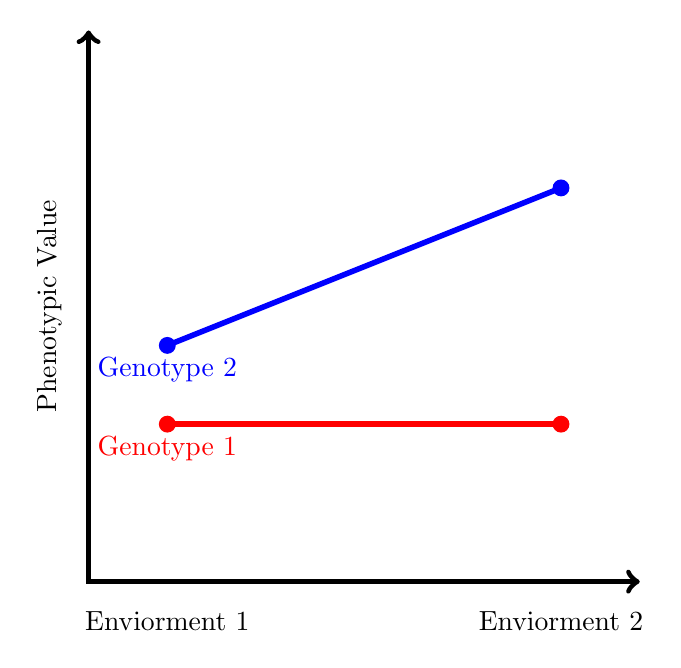
\begin{tikzpicture}
	% axes
	\draw[line width=2, black, <->] (7,0)  -- (0,0) --(0,7);

	% interaction
	\draw[line width=2, red] (1,2) node[below] {Genotype 1}-- (6,2);
	\draw[red, fill=red] (1,2) circle (0.1cm);
	\draw[red, fill=red] (6,2) circle (0.1cm);

	\draw[line width=2, blue] (1,3) node[below] {Genotype 2}-- (6,5);
	\draw[blue, fill=blue] (1,3) circle (0.1cm);
	\draw[blue, fill=blue] (6,5) circle (0.1cm);

	% text
	\node at (1,-0.5) {Enviorment 1};
	\node at (6,-0.5) {Enviorment 2};
	\node[rotate=90] at (-0.5,3.5) {Phenotypic Value};
\end{tikzpicture}
}
    \caption{Gene-by-Enviorment interaction}\label{fig:gene_env_interaction}
  \end{subfigure}
  \caption[Gene-Environment Interactions]{Different interactions between genes and the environment. 
    The colors represent different genotypes. 
    (a) Plasticity. Different environments results in the same effect independent of genotypes.
    (b) Gene-by-Environment Interaction. The effect of the environment is genotype specific}\label{fig:env_interactions}
\end{figure}

\subsection{\textit{MAOA} interactions}
\label{sub:maoa_interactions}

The effects of \textit{MAOA} and serotonin transporters have been show to be dependent on the individuals previous experiences.
\citet{Caspi2002} showed in a sample of $499$ male children that some children who were maltreated developed anti-social behavior.
This effect seemed to be moderated by a mutation in \textit{MAOA}.
Children with higher expression of \textit{MAOA} were less likely to suffer from anti-social behavior following maltreatment.
These results were later replicated by a number of similar studies~\cite{KimCohen2006}.
However, not all studies were able to replicate these findings.
\citet{Anholt2012} suggested that the failure to replicate can be explained by the low statistical power of some of the studies as well as diversity of the used samples, including sex, age and ethnicity.
Indeed, other studies have found a more complex picture of \textit{MAOA}-environment interactions.
\citet{Huang2004} for example showed that this gene-environment interaction is male specific, and \citet{Weder2009} demonstrated that extrem cases of maltreatment did not result in varying effects of later anti-social behaviors.
Nevertheless, it is still unclear how maltreatment in childhood results in anti-social behavior later in life and how \textit{MAOA} is moderating this effect.
Further, most studies have little statistical power.
Thus large scale population data is necessary to confirm this gene-by-environment interaction.

\subsection{\textit{5-HTTLPR} interactions}
\label{sub:httlpr_interactions}
Interestingly, also the serotonin transporter has been subject to investigations regarding gene-environment interactions.
However, the results are less conclusive.
Polymorphism in \textit{5-HTTLPR} have been found to result in higher levels of aggressive behaviors in a people with depression~\cite{Gonda2011}, and intellectual disabilities~\cite{May2010} while not demonstrating associations in non-affected subjects.
In the review by~\citet{Anholt2012} the authors suggested these associations as a further indicator for gene-environment interactions.
However, given the low sample size of the studies other possibilities might be possible as well.
For example shared genetic mechanism between depression, intellectual disabilities and aggression could also explain the increased effect of polymorphism in \textit{5-HTTLPR} on aggressive behavior. 
Nevertheless, the identification of gene-environment interaction within aggressive behavior suggest a complicated genetic architecture underlying aggressive behavior.
\bigskip

In conclusion, I have outline definitions of aggressive behavior and evolutionary theories and concepts surrounding it.
Further, I have reviewed and described previous research into specific genetic aspects of aggression in human and nonhuman animals alike.
In addition I have shown that previous research has also demonstrated considerable gene-environment interaction within aggression.
In the following chapter I will describe methods used to investigate the genetic architecture of human aggression.

\chapter{General Methodology}
\label{cha:methods_applied_in_genetic_studies_on_humans}

The investigation of underlying genetic architecture of human traits is limited to non-experimental studies and one can broadly distinguish between two types: twin studies and association studies.
Twin studies make use of monozygotic and dizygotic twin pairs to estimate the contribution of genetic and environmental components of a trait.
In contrast, association studies make use of recently developed molecular methods to identify specific genetic variation within the human genome associated with a specific trait.
Within this section I will describe commonly used methods in both twin and molecular based association studies.
I will further describe methods used to estimate heritability and genetic correlations.

\section{Twin Studies}
\label{sec:twin_based_studies}

Twins have always been of special interest to scholars.
Indeed already Hippocrates has been reported to be interested in twins at around 5th century BCE\@.
While his original accounts are lost, the Roman politician and author Cicero described Hippocrates's observations of two ill brothers, suspected to be twins, with similar identical disease progression~\cite{Cicero44BC},
thus providing the first written account of a twin study.

Much later Francis Galton was one of the first persons to use twins in order to investigate the effect of genes and the environment on human behavior~\cite{Rende1990}.
However, only when~\citet{Simens1924} discovered the two distinct types of twins, namely \acrfull{mz} and \acrfull{dz} twins, twin studies became an established instrument in the investigation of genetic factors in humans.

MZ twins develop from a single fertilized egg and therefore share all of their genetic makeup.
On the other hand, \acrshort{dz} twins develop from two fertilized eggs and share only 50\% of segregating genetic variants.
This distinction forms the basis of all twin studies and allows use of structural equations relating observed trait and theorized underlying genetic and environmental effects.

In addition, genetic effects can be further distinguished between additive genetic effects (A) which represent the accumulated effect of all genetic variations and dominant (D) effects which represents interaction on the same genetic locus.
Environmental components are differentiated into shared environment (C) and unique environment (E).
Therefore, the total variance of any particular trait is $P = A+D+C+E$.

Since one can assume different correlations between MZ ($r_{MZ}$) and DZ ($r_{DZ}$) twin pairs one can estimate components of $P$.
While the correlations between twins within C and E are the same in both MZ and DZ twins, namely $1$ and $0$, respectively,
MZ twins have a correlation of $1$ for both A and D, while DZ pairs have a correlation of $\frac{1}{2}$ and $\frac{1}{4}$, respectively.
Therefore differences within MZ twins can be attributed to E alone.
Further, when we assume that DZ and MZ twins are exposed to the same degree of similarity within their environment, the differences in similarity between MZ and DZ twins is an estimate of all the genetic contribution to the phenotypic variance (i.e. including additive, dominant, and epistatic effects).
This is also called Falconer's formula (see Formula~\ref{eq:falcon}) and can be used to estimate broad sense heritability, also denoted as $H^2$:
\begin{align}
  H^2 &= 2(r_{MZ}-r_{DZ}) \label{eq:falcon} \\ 
  C &= r_{MZ} - H^2  \\
  E &= 1 - r_{MZ}  
\end{align}

However, while the above is attractive it its simplicity, today's twin studies use \acrfull{sem} to model genetic and environment effects.
SEM is more flexible in modeling specific hypotheses, such as testing for sex differences as well  handling multivariate data~\cite{Rijsdijk2002}.

Figure~\ref{fig:ace} displays such a classical path-based model.
Variables within a SEM can be separated into latent and observed variables.
Additive genetic (A), common environment (C) and unique environment (E) are  latent variables.
These variables are not directly observed but are inferred from actual measured variables.
Observed variables are commonly displayed in cornered boxes.
The correlations among A and C are represented by the double headed arrows.
The causal paths $a$, $c$, and $e$ represent the effect of the components on the trait $T$, and the square of these estimates represent the variance accounted for by each of the corresponding latent factors.
However, effects of $D$ cannot be simultaneously estimated with $A$, and two separate models need to be constructed.

\begin{figure}[htpb]
  \centering
  \scalebox{0.6}{%\usetikzlibrary{external}
%\tikzset{external/system call={latex \tikzexternalcheckshellescape -halt-on-error
%		-interaction=batchmode -jobname "\image" "\texsource";
%		dvips -o "\image".ps "\image".dvi ;
%		ps2eps "\image.ps" "\image".eps}}
%\tikzexternalize
%\newcommand{\at}{\makeatletter @\makeatother}
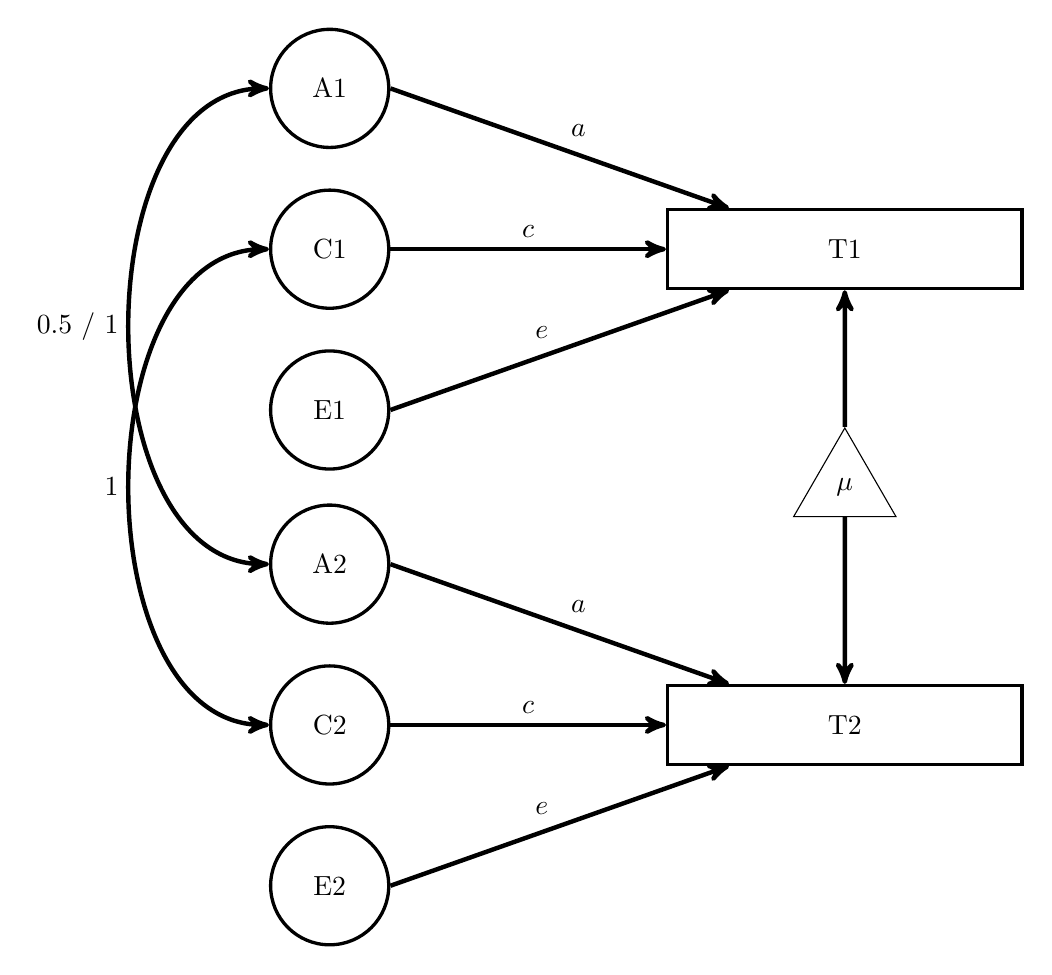
\begin{tikzpicture}[auto,node distance=.5cm,
    latent/.style={circle,draw,very thick,inner sep=0pt,minimum size=15mm,align=center},
    manifest/.style={rectangle,draw,very thick,inner sep=0pt,minimum width=45mm,minimum height=10mm},
    paths/.style={->, ultra thick, >=stealth'},
    twopaths2/.style={<->, ultra thick,bend left=90, >=stealth'},
    twopaths1/.style={<->, ultra thick,bend right=90, >=stealth'},
    mean/.style={draw, regular polygon, regular polygon sides=3, node distance=1cm, minimum height=15mm}
]

% Define observed variables
\node [manifest] (T1) at (0,0) {T1};
\node [manifest] (T2) [below=of T1, below=5cm of T1]  {T2};


% Define latent variables
\node [latent] (C1) [left=3.5cm of T1] {C1};
\node [latent] (C2) [left=3.5cm of T2] {C2};
\node [latent] (A1) [above=of C1] {A1};
\node [latent] (A2) [above=of C2] {A2};
\node [latent] (E1) [below=of C1] {E1};
\node [latent] (E2) [below=of C2] {E2};

\node [mean] (mu) at($(T1)!0.5!(T2)$)  {$\mu$};

% paths to T1/T2
\draw [paths] (A1.east) to node {$a$} (T1);
\draw [paths] (A2.east) to node {$a$} (T2);
\draw [paths] (C1.east) to node {$c$} (T1);
\draw [paths] (C2.east) to node {$c$} (T2);
\draw [paths] (E1.east) to node {$e$} (T1);
\draw [paths] (E2.east) to node {$e$} (T2);

% path from mean
\draw [paths] (mu.south) to node [right] {} (T2);
\draw [paths] (mu.north) to node [right] {} (T1);

% variance
\draw [twopaths1] (A1.west) to node  [bend left=90, left]{0.5 / 1} (A2.west);
\draw [twopaths2] (C2.west) to node  [bend right=90, left]{1} (C1.west);

\end{tikzpicture}
}
  \caption[ACE Model]{
    Basic ACE model.
    This basic model contains the latent variables A, C and E for twin 1 and 2, as well as the observed variable T with the mean $\mu$.
  }\label{fig:ace}
\end{figure}

The covariance matrix of the model in Figure~\ref{fig:ace} is therefore
\begin{equation}
  cov(MZ) = 
  \begin{pmatrix}
    a^2 + c^2 + e^2 & a^2 + c^2 \\
    a^2 + c^2 & a^2 + c^2 + e^2
  \end{pmatrix}
\end{equation}
and 
\begin{equation}
  cov(DZ) = 
  \begin{pmatrix}
    a^2 + c^2 + e^2 & \frac{1}{2}a^2 + c^2 \\
    \frac{1}{2}a^2 + c^2 & a^2 + c^2 + e^2
  \end{pmatrix}
\end{equation}
Modern SEM software are able to estimate parameters by minimising the goodness-of-fit statistic between the observed and predicted covariance matrices~\cite{Boker2011}.
Most commonly this is done via a maximum-likelihood function.
Furthermore, the overall goodness-of-fit of the model relative to a perfect fit, meaning that all covariances are estimated, is measured by a likelihood ratio square statistic ($\chi^2$).
Therefore, should we fail to reject the null hypothesis that our model in Figure~\ref{fig:ace} is different from a perfect fitted model we have reason to assume that our genetic model fits the data.

The use of SEM allows for great flexibility and a variety of models to be estimated.
In the past few decades numerous twin studies on a variety of traits have been performed.
It not only allowed testing for the differences in the genetic architecture between the sexes but also examining how influence of genetic factors change over age.
However, due to the new advances in molecular technology,  more research has  shifted to \acrfull{gwas}.
Hence, in the next section I will outline the methods applied in GWAS\@.

\section{Association Studies of Common Variants}
\label{sec:association_studies_of_common_variants}

Large-scale genomic association studies have enabled researchers to investigate specific genetic factors associated with a certain trait.
Hence, while twin studies were only able to give an estimate of the total contribution of genetic factors on a phenotype, association studies are able to elucidate the specific molecular basis of complex traits.
Specifically, these genome-wide association studies utilize common \acrfull{snp} and other genetic variants, to identify specific genetic markers associated with a certain trait.
Common variants are usually genetic variations with a frequency $\ge 1\%$, also called \acrfull{maf}.

\paragraph{What is a \acrfull{snp}}
\label{par:what_are_snp}
SNPs are variations within the genome at  specific positions and may underly differences in traits and disease susceptibility. 
For example, the replacement of the nucleotide cytosine (C) with thymine (T) at a certain position within a stretch of DNA is considered a \acrfull{snp}.

Association analysis of common genetic variants is usually only applied to investigate potential genetic markers of common traits and disorders, while different strategies are applied for rare diseases.
Indeed assessments of families whose members are disproportional affected with a rare genetic disorder, such as Huntigton's disease or cystic fibrosis, were able to identify a number of disease-causing variants~\cite{Kerem1989}.
However, while this method was initially successful with a number of other rare disorders, common disorders, such as heart disease, psychiatric disorders, as well as others, fared not that well,  
implying that common and rare disorders have a different genetic architecture~\cite{Hirschhorn2005a}.
This resulted in the conceptualization of the common disease common variant hypothesis.


\subsection{Common Disease Common Variant Hypothesis}
\label{sub:common_versus_rare_genetic_variants}

The common disease common variant hypothesis suggests that common disorders are affected by genetic variations which are also common in the population~\cite{Schork2010}.
This hypothesis, while simplistic, has some profound implications.

Importantly it is unlikely that common variants will have a high penetrance and are the lone disease-causing mutations.
For example, a common variant with a frequency of 45\% that directly causes a disorder would mean that also 45\% of the population would be affected by the disease.
This is unlikely to be the case and it is more likely that a given SNP only has a small effect on the disease.
This in turn also implies that multiple common variants affect a common disorder.
For example, twin studies have estimated the heritability of aggressive behavior at 50\%.
If a single SNP has only a small effect on the phenotype, then the total genetic risk must be distributed across multiple common genetic variants.
Figure~\ref{fig:rare_comon} displays the spectrum of genetic affects and allele frequency.
\begin{figure}[htpb]
  \centering
  \includegraphics[width=0.8\linewidth]{{introduction/figure/journal.pcbi.1002822.g001}.png}
  \caption[Spectrum of Disease Allele Effects]{Spectrum of Disease Allele Effects~\cite{Bush2012}.}\label{fig:rare_comon}
\end{figure}

Overall, the common disease common variant hypothesis has been tested numerous times~\cite{Bush2012}.
Most common SNPs identified in the last 10 years are of small effect and most common disorders have multiple risk alleles~\cite{Welter2014,Schork2010}, suggesting that the hypothesis holds true. 
However this does imply that all genetic contributions to a common disorder are due to common variants alone.
Indeed, there have been some successful genetic associations of common variants in rare disorders.
For example,~\cite{Garcia-Barcelo2009a} identified 2 common SNPs associated with Hirschsprung's disease, a rare congenital disorder (2.8 per 10,000 births).

\subsection{Linkage Disequilibrium}
\label{sub:linkage_disequilibrium}

Before explaining the concept of association studies in more detail it is important to mention \acrfull{ld}.
LD is `the nonrandom association of alleles at different loci'~\cite{Slatkin2008} and forms a marker of the population genetic mechanism that is at play within our genome.
For example, two loci are said to be in high LD when allele $A$ at one loci co-occurs with allele $B$ at a different loci at a higher frequency then one would expect if the two loci were independent.
Hence the level of LD can be quantified as $D_{AB}=p_{AB} - p_{A}p_{B}$ in which in which $p_{AB}$ is the frequency that $A$ and $B$ occurs together wile $p_A$ and $p_B$ is the frequency of $A$ and $B$, respectively.
If $D_{AB} \neq 0$, A and B are said to be in linkage disequilibrium, otherwise the two alleles are in linkage equilibrium ($D_{AB}=0$).
Nevertheless, $D_{AB}$ depends on the frequencies of the alleles in questions and is therefore not always convenient.
Therefore, LD between two loci is commonly measured in two different ways. 
That is $D'$ and $r^2$.
\citet{Lewontin1964} suggested to use
\begin{equation}\label{eq:dprime}
  D' = D/D_{\min}
\end{equation}
where 
\begin{equation*}
  D_{\min}= \begin{cases}
    \max\{-p_A p_B,\,-(1-p_A)(1-p_B)\} & \text{when } D < 0\\
    \min\{p_A (1-p_B),\,(1-p_A) p_B\} & \text{when } D > 0
  \end{cases} 
\end{equation*}
Alternatively, one can also use the correlation coefficient $r$ between the two loci 
\begin{equation}\label{eq:r2}
  r=\frac{D}{\sqrt{p_A(1-p_A)p_B (1-p_B)}}
\end{equation}
An important consequence for association studies is that when an association between a trait and an allele is found, that allele is unlikely to be the actual causal SNP\@.
An association between a SNP and a trait can arise for multiple reasons.
First, the association could represent the true effect and the particular SNP has a causal relationship on the trait in question.
Second, and more likely, the associated SNP is a proxy of the causal SNP since both are in high \acrshort{ld}.
Third, the association is a random fluctuation within the sample, and 
fourth, the association is due to confounding errors such as population stratification or genotyping errors.

\subsection{Association Test}
\label{sub:association_test}

The association between a SNP $g$ and a trait $y$, as well as additional $p$ covariates $\bm{U}$, of an individual $i$ can be expressed as a generalized linear regression model for a continuous or binary phenotype:
\begin{equation}
  g(E(y_i)) = \beta_0 + \beta_1g_i + \bm{\beta_u}\bm{U_i'} + \epsilon
\end{equation}
in which $\beta_0$ is the intercept (commonly ignored in GWAS settings) and $\beta_1$ the regression coefficient of a particular SNP\@.
The vector $\bm{\beta_u}$ of size $1\times p$ are the regression coefficients of $p$ covariates to adjust for potential confounding factors.
Possible confounding factors are population stratification, sex, genotyping chip, and others.
The link function $g(.)$ is a logit function for binary traits, while for quantitative traits no transformation is used (identity link function). 

Genotypes of each SNP can be organized to represent dominant, recessive, multiplicative, as well as additive models~\cite{Bush2012}.
For example, assuming at a given position the two genotypes are \textit{A} and \textit{a}.
In a dominant model (for \textit{A}) disease risk increases for having one or two copies of \textit{A} over no copies of \textit{A}.
Thus the risk $k$ is the same for \textit{Aa} and \textit{AA}.
In contrast, a recessive model (for \textit{A}) requires at least two copies of the risk allele \textit{A}.
The multiplicative model (for \textit{A}) expects a squared increase in risk.
If the risk of having the \textit{A} allele is $k$ then the risk of two copies of the same allele is $k^2$.
An additive model assumes a linear increase in risk for each additional allele copy.
Thus if the risk of \textit{Aa} is $k$ then the risk doubles ($2k$) for \textit{AA}. 
Despite these different models, GWAS commonly uses an additive model only since it has appropriate statistical power to detect dominant effects as well.
Nevertheless, an additive model has reduced power for potential recessive effects~\cite{Bush2012}.

\subsection{Population Stratification}
\label{ssec:population_stratification}

Population stratification takes place when differences in the frequencies of alleles among cases and controls are not due to a causal relationship between the SNP and the trait.
Rather, they are caused by ancestral differences across populations.
An association is affected by population stratification if the trait is more prevalent in one population while the allele frequencies vary across the populations.

Commonly one can adjust for population stratification by the usage of \acrfull{pca}.
PCA is a procedure which transforms a set of correlated variables into a set of linear uncorrelated ones, called principle components (\acrshort{pc}).
The number of PC can be smaller or equal to that of the number of initial variables and the first PC accounts for most of the variability in the set of correlated variables.
Each following PC explains the most variance constrained that it is orthogonal to the previous.

Using PCA on a matrix of individuals by SNPs, in which each cell represents the count of minor alleles, results in a set of PCs which explain the genetic variation within the sample.
Given the sample is a mixture out of multiple populations with different ancestry the computed PCs will often have geographic interpretation.
Thus including PCs into the association model will adjust for population stratification arising due to differences in allele frequencies and disease prevalence.

\subsection{Multiple Testing}
\label{ssec:multiple_testing}

Testing a large number of genetic variants without adjusting the significance threshold $\alpha$ results in a large number of falsely associated variants.
Therefore, adjustment of the significance threshold is necessary.
For example, one could simply adjust $\alpha$ by the number of tests performed (Bonferroni threshold).
However, this would result in an overly conservative threshold and in a number of false negative associations~\cite{Benjamini1995} since computed test statistics are not independent due to LD\@.
Indeed,~\citet{Peer2008} estimated, based on data from the International Haplotype Map Consortium, the number of independent tests to be one million in Europeans and two million in African populations.
Therefore most GWAS have used a threshold of $5\times 10^{-8}$.
However, due to the introduction of larger sample sizes as well as better technology we are able to genotype variants with lower allele frequency.
This requires more stringent adjustment of the GWAS significant threshold since it also increases the number of independent tests.
Hence~\citet{Fadista2016} recently suggested to use $3\times10^{-8}$, $2\times10^{-8}$, $1\times10^{-8}$ when including variants with $MAF\ge1\%$, $MAF\ge0.5\%$, and $MAF\ge0.1\%$, respectively.

\acrshort{gwas} are useful in identifying molecular markers for traits and diseases.
While there are multiple possible confounding factors, such as population stratification, methods have been developed to approach these problems successfully.


\section{Heritability and Genetic Correlation}
\label{sec:heritability_and_genetic_correlation}

As already described above, studies on twins were able to assess the heritability of traits by considering the MZ and DZ twin correlations.
Interestingly, a number of methods have also been developed to assess narrow sense heritability, or the additive genetic effect, from genotyped data.
Several methods have been proposed in the past, most notably \acrfull{gcta} and LD-score regression.

\subsection{\acrfull{gcta}}
\label{sub:gcta}

GCTA uses a mixed linear model to  fit the effect of all SNPs by making use of the genetic relationship matrix of all included subjects~\cite{Yang2011}.
If $\textbf{A}$ is the genetic relatedness matrix then
\begin{equation}
  y = X\beta + g + \epsilon \text{ with } var(y) = V = A\sigma^2_g + I\sigma^2_\epsilon
\end{equation}
in which $y$ is the phenotype and $\beta$ are the estimated effect sizes of all covariates and the total genetic effect $g$ for each individual is $g \sim N(0, A\sigma^2_g)$.
GCTA is then able to estimate the variance explained by all SNPs, $\sigma^2_g$, by restricted maximum likelihood.
One can extent this model to bivariate linear mixed models to estimate the genetic correlation between two traits as well.
If $y_1 = X_1\beta_1 + g_1 + \epsilon_1$ for trait 1 and $y_2= X_2\beta_2 + g_2 + \epsilon_2$ for trait 2 then the variance-covariance matrix $V$ is
\begin{equation}
  V = 
  \begin{pmatrix}
    Z_1AZ_1'\sigma_{g1} + I\sigma^2_{\epsilon 1} & Z_1AZ_2'\sigma_{g_1g_2} \\
    Z_2AZ_1'\sigma_{g_1g_2} & Z_2AZ_2'\sigma_{g2} + I\sigma^2_{\epsilon 2}
  \end{pmatrix}
\end{equation}
in which $X$ and $Z$ are the incidence matrices for the effects of $\beta$ and $g$.
However, GCTA requires considerable computational power as well as the availability of the raw genotype data.
Hence LD-score regression has been developed to estimate heritability on summary statistics only.

\subsection{LD-score Regression}
\label{sub:ld_score_regression}

LD-score regression makes use of the previously outlined LD among tagged and causal SNPs.
Test statistics of SNPs in high LD with the causal variant will be elevated proportional to their LD\@.
Thus the more genetic variation a SNP tags the higher the probability that it will tag a causal variant.
LD-score regression makes use of this relationship and regresses the estimated $\chi^2$ from the association study on the LD-score, which measures the overall LD of variant $j = 1, \ldots, M$ as $\ell_j = \sum^M_{k=1} r^2_{jk}$. 
The slope of this regression can then be interpreted as an estimate of heritability~\cite{Bulik-Sullivan2015}.
Similarly, if we replace the $\chi^2$ of a single study by the product of the z-scores of two separate studies and regress it onto $\ell_j \sqrt{N_{1}N_{2}}$, the slope can be interpreted as the genetic covariance between trait 1 and 2~\cite{Bulik-Sullivan2015a}.

\section{The Missing Heritability}
\label{sec:missing_heritability}

One would expect that the variance explained by all genetic variants combined would result in similar estimates as to those estimated in twin studies.
Unfortunately, for many traits, this is not the case.
This is called the `Missing Heritability Problem'~\cite{Vineis2010} and a  number of reasons have been suggested for the discrepancy between estimates in twin studies and those in GWAS\@.

First, the assumptions in twin studies might be violated and estimates are too high.
In particular, studies on twins assume that shared environmental factors influence MZ and DZ twins to the same extent.
However, one can argue that MZ twins are treated by parents, teachers, and peers differently resulting in a potential violation of the this equal environments assumption. 
However, while previous research suggest that the equal environment assumption might not be strictly valid, the induced bias is likely to be small~\cite{Derks2006,Felson2014}

Second, GWAS only consider common variants and rare variants might account for the missing heritability.
While most rare variants have little or no effect on traits, some rare variants have very large effects.
Indeed, a study on height found that while most common variants only had small effects, some rare genetic variants resulted in a large increase in height of up to $2cm$~\cite{Marouli2017}.
This would indicate that rare variants can have a profound effect on common traits, suggesting that heritability estimates using common variants alone might be biased downward.

Third, epistasis is only insufficiently captured in most studies and could account for the differences.
Indeed, many twin concordance rates indicate the presence of non-additive effects to some extent.
Further, complex gene-gene interaction have been shown in a number of experimental studies in  animals~\cite{Zuk24012012}.
Therefore suggesting that epistatic effects might play a major role in humans as well.
However, models which include gene-gene or even gene-gene-gene and higher order interactions are very computational intensive and require large datasets~\cite{Lippert2013}. 

Fourth, gene regulatory components, such as RNA expression and methylation, might explain the discrepancy between estimates.
Methods investigating regulatory components have only been recently introduced for large-scale population analysis and alteration of gene expression by epigenetic modifications could be heritable without affecting the underlying DNA sequence~\cite{Trerotola2015,Nadeau2009}.
Indeed, various studies have shown that some environmental factors can lead to epigentic changes that can be carried over to following generations without continued exposure~\cite{Nadeau2009,Skinner2011}.
This separate model of inheritance, next to Mendelian heredity, would be undetectable in GWAS\@.

While a single reason for the missing heritability seems unlikely it is still an ongoing research objective to account for the differences.

\subsection{Genetic Correlations}
\label{sub:genetic_correlations_method}
The development of both LD-score regression and GCTA have enabled recent research to uncover the genetic correlations among a variety of different traits, even when the two traits are measured on different people.
However, genetic correlation can arise from a multitude of different sources.
Figure~\ref{fig:genetic_correlation} shows 4 different ways genetic correlation can arise.
First and foremost, genetic correlation can arise if two traits are caused by the same genetic factors (see Figure~\ref{fig:pleiotropy}).
Second, a genetic factor  causes phenotype 1 and that phenotype can in turn cause phenotype 2 (see mediated pleiotropy in Figure~\ref{fig:mediated_pleiotropy}).
Third, genetic correlation can also arise from assortative mating as shown in Figure~\ref{fig:assortative_mating}.
Assortative mating is a non-random mating pattern within a population.
For example, consider two traits which share no causal variant.
Trait 1 is desirable in males while trait 2 is desirable in females.
Over a few generation this will result in LD between causal variants of trait 1 and 2 despite sharing no initial causal SNPs, resulting in a genetic correlation. 
Fourth, also parental effect can result in genetic corrections as displayed in Figure~\ref{fig:parental_effects}.
Specifically, genetic components cause trait $1$ in the parents which influences the child's environment which in turn results in trait 2. 
Nevertheless, the genetic correlations estimated by LD-score and GCTA are unable to distinguish between the possible sources of genetic correlations.

\begin{figure}[htp]
  \begin{subfigure}[t]{0.4\textwidth}
    \centering
    \resizebox{0.5\linewidth}{!}{\input{introduction/figure/genetic_correlation/pleiotropy.tex}} 
    \caption{Pleiotropy}\label{fig:pleiotropy}
  \end{subfigure}
  \begin{subfigure}[t]{0.4\textwidth}
    \centering
    \resizebox{0.5\linewidth}{!}{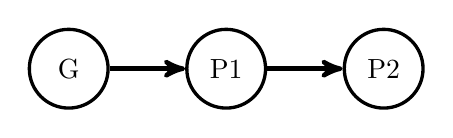
\begin{tikzpicture}[auto,node distance=.5cm,
    latent/.style={circle,draw,very thick,inner sep=0pt,minimum size=10mm,align=center},
    manifest/.style={rectangle,draw,very thick,inner sep=0pt,minimum width=45mm,minimum height=10mm},
    paths/.style={->, ultra thick, >=stealth'},
    twopaths2/.style={<->, ultra thick,bend left=90, >=stealth'},
    twopaths1/.style={<->, ultra thick,bend right=90, >=stealth'},
    mean/.style={draw, regular polygon, regular polygon sides=3, node distance=1cm, minimum height=10mm}
]

\node [latent] (G) at  (0,0) {G};
\node [latent] (P1) at (2,0) {P1};
\node [latent] (P2) at (4,0) {P2};

\draw [paths] (G.east) to node [right] {} (P1);
\draw [paths] (P1.east) to node [right] {} (P2);

\end{tikzpicture}
} 
    \caption{Mediated Pleiotropy}\label{fig:mediated_pleiotropy}
  \end{subfigure}
  \begin{subfigure}[t]{0.4\textwidth}
    \centering
    \resizebox{0.6\linewidth}{!}{
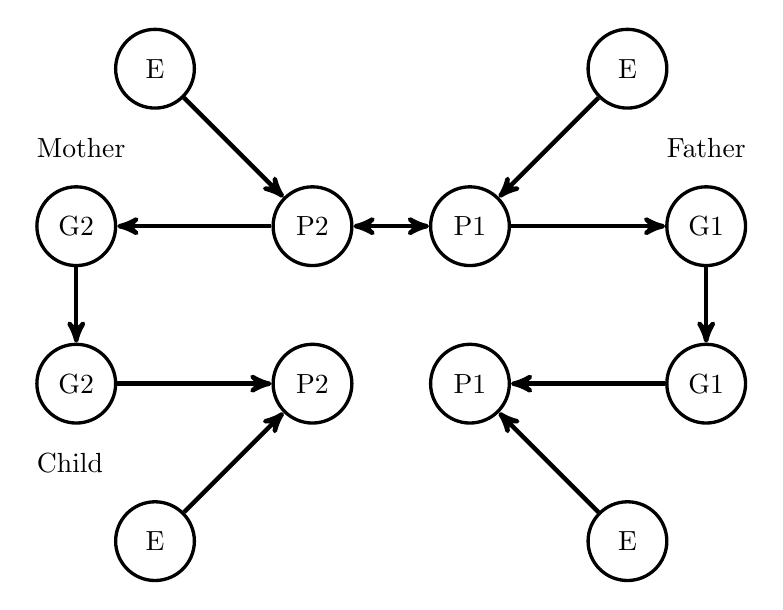
\begin{tikzpicture}[auto,node distance=.5cm,
    latent/.style={circle,draw,very thick,inner sep=0pt,minimum size=10mm,align=center},
    manifest/.style={rectangle,draw,very thick,inner sep=0pt,minimum width=45mm,minimum height=10mm},
    paths/.style={->, ultra thick, >=stealth'},
    paths2/.style={<->, ultra thick, >=stealth'},
    twopaths2/.style={<->, ultra thick,bend left=90, >=stealth'},
    twopaths1/.style={<->, ultra thick,bend right=90, >=stealth'},
    mean/.style={draw, regular polygon, regular polygon sides=3, node distance=1cm, minimum height=10mm}
]

\node [latent] (P2) at (0,0) {P2};
\node [latent] (P1) at (2,0) {P1};

\node [latent] (G1) at (5,0) {G1};
\node [latent] (G2) at (-3,0) {G2};

\node [latent] (E1) at (4,2) {E};
\node [latent] (E2) at (-2,2) {E};

\node [latent] (P1c) at (2,-2) {P1};
\node [latent] (P2c) at (0,-2) {P2};

\node [latent] (G1c) at (5,-2) {G1};
\node [latent] (G2c) at (-3,-2) {G2};

\node [latent] (E1c) at (4,-4) {E};
\node [latent] (E2c) at (-2,-4) {E};

\draw [paths] (P1.east) to node [right] {} (G1);
\draw [paths] (P2.west) to node [right] {} (G2);
\draw [paths] (G1.south) to node [right] {} (G1c);
\draw [paths] (G2.south) to node [right] {} (G2c);
\draw [paths] (E1.south west) to node [right] {} (P1);
\draw [paths] (E2.south east) to node [right] {} (P2);

\draw [paths] (G1c.west) to node [right] {} (P1c);
\draw [paths] (G2c.east) to node [right] {} (P2c);

\draw [paths] (E1c.north west) to node [right] {} (P1c);
\draw [paths] (E2c.north east) to node [right] {} (P2c);

\draw [paths2] (P1.west) to node [right] {} (P2.east);


\node [text width=1cm] at (5,1) {Father};
\node [text width=1cm] at (-3,1) {Mother};
\node [text width=1cm] at (-3,-3) {Child};

\end{tikzpicture}
} 
    \caption{Assortative Mating}\label{fig:assortative_mating}
  \end{subfigure}
  \begin{subfigure}[t]{0.4\textwidth}
    \centering
    \resizebox{0.6\linewidth}{!}{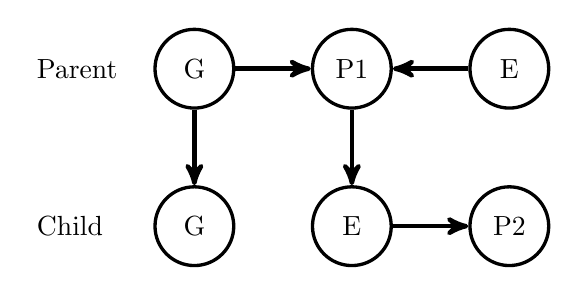
\begin{tikzpicture}[auto,node distance=.5cm,
    latent/.style={circle,draw,very thick,inner sep=0pt,minimum size=10mm,align=center},
    manifest/.style={rectangle,draw,very thick,inner sep=0pt,minimum width=45mm,minimum height=10mm},
    paths/.style={->, ultra thick, >=stealth'},
    twopaths2/.style={<->, ultra thick,bend left=90, >=stealth'},
    twopaths1/.style={<->, ultra thick,bend right=90, >=stealth'},
    mean/.style={draw, regular polygon, regular polygon sides=3, node distance=1cm, minimum height=10mm}
]

\node [latent] (Gp) at (0,0) {G};
\node [latent] (P1) at (2,0) {P1};
\node [latent] (Ep) at  (4,0) {E};
\node [latent] (Gc) at (0,-2) {G};
\node [latent] (Ec) at  (2,-2) {E};
\node [latent] (P2) at (4,-2) {P2};

\node [text width=1cm] at (-1.5,0) {Parent};
\node [text width=1cm] at (-1.5,-2) {Child};

\draw [paths] (Gp.east) to node [right] {} (P1);
\draw [paths] (Gp.south) to node [right] {} (Gc);
\draw [paths] (P1.south) to node [right] {} (Ec);
\draw [paths] (Ep.west) to node [right] {} (P1);
\draw [paths] (Ec.east) to node [right] {} (P2);

\end{tikzpicture}
}
    \caption{Parental Effects}\label{fig:parental_effects}
  \end{subfigure}
  \caption[Sources of Genetic Correlations]{Different sources of genetic correlation according to~\citet{Pickrell2016}}\label{fig:genetic_correlation}
\end{figure}

To conclude, during the last few years large gains have been made in fostering our understanding of heritability and genetic correlations with the development of GCTA and LD-score regression.
While these tools are able to estimate heritability and genetic correlations of a number of traits it remains difficult to distinguish between different sources of genetic correlations.

\section{Association Studies on Rare Variants}
\label{sec:association_studies_on_rare_varitants}

A possible suspect for the missing heritability are rare variants.
Rare variants,  variants with a \acrfull{maf} of 1\% or lower, have been suggested to explain the bulk of missing heritability~\cite{Jiang2013,Li2009a}.
Rare variants are commonly not accessible via micro array chips but only via the more cost intensive sequencing.
However, the drop in sequencing costs has allowed us to conduct whole-exome and whole genome association studies of rare variants~\cite{Goodwin2016}.
In contrast to GWAS, single variant associations are largely unfeasible, unless sample size is very large~\cite{Lee2014}.
Hence, considerable effort has been made to develop and deploy statistical methods to improve statistical power of rare variant association studies~\cite{Morris2010,Zeng2014,Daye2012,Manuscript2013}.
Instead of testing individual genetic markers most statistical tests evaluate the combined effect of multiple genetic variations in a biologically-relevant region, such as a gene.
In general, one can divide such approaches into burden and variance component tests.
I will first introduce the general statistical model for the two tests.
Following, I will outline two commonly used classes of tests and evaluate their benefits and drawbacks.

Assuming that $y_i$ for subject $i$ with mean $\mu_i$ follows a distribution in the quasi-likelihood family~\cite{Lee2014} with $n$ subjects in a region with $m$ variants, then
\begin{equation}
  h(\mu_i) = \alpha_0 + \alpha'X_i +\beta'G_i
\end{equation}
in which $h(\mu) = \mu$ or $h(\mu) = logit(\mu)$.
The regression coefficients of the covariates and allele counts are $\alpha = (\alpha_1, \ldots, \alpha_q)$ as well as $\beta = (\beta_1, \ldots, \beta_m)$, respectively.
The covariates are denoted as $X_i = (X_{i1}, \ldots, X_{iq})'$ and the allele counts as $G_{i1}, \ldots, G_{im}$.
The score statistic of the marginal model for variant $j$ is then
\begin{equation}
  S_j = \sum^n_{i=1} G_{ij}(y_i-\hat{\mu_i})
\end{equation}
where $\hat{\mu_i}$ is the estimated mean under $H_0: \beta = 0 $ and is obtained by $h(\mu_i) = \alpha_0 + \alpha'X_i$.

\subsection{Burden Test}
\label{sub:burden_test}
The simplest approach, called the burden test, tests the weighted sum of computed scores:
\begin{equation}\label{eq:burden}
  Q = {(\sum^{m}_{j=1} w_{j} S_{j})}^2
\end{equation}
in which $w_j$ is the weight for variant $j$.
Weights can be define by functional annotations, allele frequency, or other means.
The test assumes that all variants  have the same direction of effect.
This is a rather strong assumption and violations result in a loss in statistical power~\cite{Derkach2013a}.

\subsection{Variance Components Tests}
\label{sub:variance_component_tests}
In contrast to burden tests, variance-components tests evaluate the distribution of effects within a certain genomic region.
The most prominent member of this test family is \acrfull{skat}~\cite{Wu2011}.
SKAT assumes that $\beta_j\sim N(0,w_j\tau)$ and tests for $H_0: \tau = 0$ with a variance-components score test.
The test statistic is defined as
\begin{equation}\label{eq:skat}
  Q = \sum^{m}_{j=1} w_{j}^2 S_{j}^2
\end{equation}
The test is robust to groupings of protective and damaging effects within the same region.
However,  SKAT suffers from a reduction in statistical power in cases of high proportions of causal variants of the same direction, as compared to the burden test~\cite{Derkach2013a}.

\section{Mendelian Randomization}
\label{sec:joint_association_study}

\subsection{General Methodology}
\label{sub:General_Methedology}

\acrfull{mr} allows  inferring potential causal effects from observational data in the presence of confounding factors. 
It allows us to assess whether a specific risk factor (exposure) has a causal effect on a disease (outcome).
MR makes use of measured variation in genetic variants with known association to a modifiable exposure, also called instrument.
Thus it assumes that certain genetic variants are associated with the exposure, and not with the outcome, except through the exposure.
Commonly, genetic variants with well known effect on the exposure are used and can be seen as a natural randomized control trial since genotypes are passed randomly from parents to offspring.
MR is based on a number of assumptions, most importantly that there is no direct relation between genetic variant and outcome as well as any other confounder.
However, the use of single variants within an MR often results in underpowered studies~\cite{Bowden2015} since the effect of an given common SNP on any phenotype is usually small.
This has led to the desire to use multiple genetic variants in order to improve statistical power to estimate causal effects between exposure and outcome.

Assume $J$ variants in $n$ subjects (indexed by $i$) were measured ($G_{i1}, G_{i2}, \ldots , G_{iJ}$),
an exposure $X_i$ ,as well as an outcome $Y_i$.
Further, the potential confounder $U_i$ is unknown. 
Within the causal model of MR the exposure is a function of the genetic variant, confounder, as well as an independent error, $\epsilon_i^X$. 
Furthermore, $\gamma_j$ represents the effect of each variant $j$ on the exposure.
The outcome, on the other hand, is the result of the linear function of the genetic variants, the exposure, the confounder, as well as an error term ($\epsilon_i^Y$).
Then the estimate of the causal effect between exposure and outcome is $\beta$, while $\alpha_j$ represents the undesired but potential direct effect between the genetic variant $j$ on the outcome:
\begin{equation} \label{eq:rm_basic}
  \begin{split}
    X_i &= \sum^J_{j=1} \gamma_jG_{ij} + U_i + \epsilon_i^X \\
    Y_i &= \sum^J_{j=1} \alpha_jG_{ij} + \beta X_i + U_i + \epsilon_i^Y \\
  \end{split}
\end{equation}
These assumed relationships of this causal model are displayed in Figure~\ref{fig:causal}.
\begin{figure}[!h]
  \centering
  \resizebox{0.5\textwidth}{!}{\begin{tikzpicture}
  \node (G) at (0,0) {$G_j$};
  \node (X) at (2,0) {$X$};
  \node (Y) at (4,0) {$Y$};
  \node (U) at (3,1) {$U$};

  \draw[black, ->] (G) -- node[below] {$\gamma_j$}(X) ;
  \draw[black, ->] (X) -- node[above] {$\beta$}(Y);
  \draw[black, ->] (U) -- (X);
  \draw[black, ->] (U) -- (Y);

  \draw[dotted, black, ->] (G) -- (U);
  \path[dotted,black, ->] (G) edge [bend right=30] node[below] {$\alpha_j$} (Y);
\end{tikzpicture}
}
  \caption[Causal Model]{Causal Model.
    Given a genetic variant $G_j$ influences the exposure $X$, it can be used as an instrumental variable to investigate the causal effect of exposure $X$ on the outcome $Y$.
    However,this model assumes that the instrumental variable $G_j$ influences the outcome $Y$ only via the exposure $X$.
    Hence assuming that $\alpha_j=0$, $\gamma_j\neq0$ and that $G_j$ does not influence $Y$ via a third variable $U$. 
    The dotted lines indicate potential assumptions violations.
  }\label{fig:causal}
\end{figure}
Should $G_j$ be independent of confounder $U$,
as well as associated with exposure $X$ and independent of outcome $y$ conditional on $X$, then variant $j$ is a valid instrument for $X$.

The reduced-form equation~\cite{Bowden2015} of Equation~\ref{eq:rm_basic}, relating outcome with $G_j$, can be written as
\begin{equation}
	\begin{split}
		Y_i &= \Gamma_j G_{ij} + \epsilon_{ij}^{'Y} \\
		&= (\alpha_j + \beta\gamma_j)G_{ij} + \epsilon_{ij}^{'Y}
	\end{split}
\end{equation}
One can then estimate the causal effect $\beta$ with the help of the Wald method~\cite{Wald1940},
by dividing the effect of variant $j$ on the outcome (denoted as $\hat{\Gamma_j}$) by the effect on the exposure (denoted as $\hat{\gamma_j}$).
Assuming that $\alpha=0$, then the causal effect $\beta$ is
\begin{equation} \label{eq:causal_estiamte}
	\beta = \frac{\beta\gamma_j}{\gamma_j}= \frac{\Gamma_j}{\gamma_j}
\end{equation}

However, single variants often have inadequate statistical power, so one can extend Equation~\ref{eq:causal_estiamte} to multiple variants as a weighted average of multiple ratio estimates across uncorrelated genetic variants~\cite{Bowden2015}:
\begin{equation} \label{eq:IVW}
  \frac{\sum^J_{j=1} \hat{\gamma}_j^2\sigma_{Yj}^{-2} \hat{\beta}_j}
  {\sum^J_{j=1} \hat{\gamma}_j^2\sigma_{Yj}^{-2}}
\end{equation}
in which $\hat{\beta}_j = \frac{\hat{\Gamma}_j}{\hat{\gamma}_j}$ and the weight $\sigma_{Yj}$ is the standard error of the outcome on the $jth$ variant.

Often one cannot assume that $\alpha_j = 0$.
In this case the Wald ratio estimate of variant $j$ will equal the true causal effect plus the error $\frac{\alpha_j}{\gamma_j}$~\cite{Bowden2015}. 
Hence in the presence of $\alpha_j \neq 0$, Equation~\ref{eq:IVW} is re-written as
\begin{equation} \label{eq:TSLSbias}
  \beta + \frac{\sum^J_{j=1} \gamma_j^2\sigma_{Y_j}^{-2} \alpha_j}
  {\sum^J_{j=1} \gamma_j^2\sigma_{Y_j}^{-2}} = \beta + Bias(\alpha, \gamma)
\end{equation}
Importantly, this implies that the assumed independence between genetic variants with the outcome $y$ conditional on $X$ holds if the bias term has a mean of zero.
Based on these general assumptions and characteristics of Mendelian randomization, numerous different methods have been proposed.

\subsection{Applied MR Methods}
\label{sub:Used_Methods}

Due to differences in robustness in regards to various potential assumption violations~\citet{Burgess2016}, it is recommended that several different MR methods be used in order to assess potential causal relationships.
The estimated causal effects can then be judged over all  applied models.
Further, a sensitivity analysis of each MR analysis can be performed to investigate validity of the underlying assumptions~\cite{Burgess2016}.
A sensitivity analysis investigates the validity of the causal inference by MR since it is implausible that all selected SNPs satisfy the instrumental variable assumption~\cite{Burgess2016}.
This is commonly done by assessing directional pleiotropy via funnel plots, investigating heterogeneity, as well as testing the reverse direction of causality and linearity.

Within this study I used five separate methods.
That is, the \acrfull{ivm}, the weighted median method, as well as MR-Egger regression~\cite{Bowden2015}.
Further I applied classical meta analysis methods with fixed~\cite{Nelson2015a} and random effects~\cite{Ahmad2015a}.
Overall, these methods differ in their robustness to pleiotropy (or the effect non-null effect of $\alpha_j$) as well as statistical power.

The IVM has been described already in the previous section (see Equation~\ref{eq:IVW}).
The method, while having greater statistical power than other methods, assumes that all used variants are valid instruments.
Thus IVM is especially susceptible to presence of pleiotropy~\cite{Burgess2015b}.
In contrast, the weighted median method first estimates the causal effect for each variant separately weighted by the inverse variance. 
Following, estimates are then ranked and the median of this distribution is used to represent the estimated causal effect between exposure and outcome.
This simple approach has the benefit that if at least 50\% of variants are valid instruments it will give consistent causal estimates.
However, this comes with a lose in precision~\cite{Bowden2015}.

MR-Egger is a newer method which relaxes the assumption of $\alpha_j=0$, instead  assuming that the correlation between $\alpha_j$ and $\gamma_j$ is $0$.
Under this assumption, the bias (see Equation~\ref{eq:TSLSbias}) is inversely proportional to $\gamma_j$ and variants with stronger instrument strength (large $\gamma_j$) will on average be closer to the true causal effect.
MR-egger makes use of this by regressing $\hat{\Gamma}_j$ on $\hat{\gamma}_j$:
\begin{equation}\label{eq:egger}
  \hat{\Gamma}_j = \beta_{0E} + \beta_{E} \hat{\gamma}_j
\end{equation}
Interestingly, $H_0$ of the intercept $\beta_E$ then gives an indication of the overall average pleiotropy.
Thus MR-egger uses a relatively relaxed assumption but comes with the cost of  considerably lower statistical power~\cite{Bowden2015}.

Finally, a fixed meta-analysis was used which assumes that the estimated effects $\beta_j$ are equal across assessed variants~\cite{Burgess2015b}.
However, this might not be the case in practice since it assumes that all selected instruments are valid.
In addition, variants might have different effects on the outcome which is not exclusively directed thought the exposure. 
In contrast, mixed-effect models do not assume equal effect across genetic variants~\cite{Burgess2015b}.
Specifically, in contrast to fixed effect model where the effect of each instrument $\beta_j$ is modeled as normally distributed with a  mean $\beta_j = \beta$ and variance $\sigma_{Y_j}^2$, a mixed-effect model assumes additionally that also $\beta_j$ is normally distributed with a mean of $\mu_\beta$ with variance $\phi^2$.

To summarise, variance-components tests are generally more powerful than burden tests if a region has many non-causal variants or when the effects of a genomic region are bi-directional.
In contrast, burden tests perform better in scenarios where most causal variants have the same direction of effect.
This has led to the development of omnibus tests to combine burden and variance component tests, most notably SKAT-O~\cite{Lee2012}.
\bigskip

To conclude, I have outlined various statistical methods to investigate the genetic contribution of aggressive behavior.
I have described the commonly applied twin model to estimate the contribution of genetic and environmental effects.
Further, I outlined the principles of genome wide association studies as well as the use of GCTA and LD-score to estimate the narrow sense heritability from common SNPs.
Finally, I have described two commonly-used rare variant tests as well as their pros and cons.

In the next chapter I will present an investigation of the longitudinal heritability of childhood aggression with the use of two large twin cohorts. 

%\documentclass[../header.tex]{subfiles}
\begin{document}
\chapter[Hertability of Aggression]{The longitudinal heritability of childhood aggression}
\label{chap:longHera}

%&tex
\chapter{Introduction}
\label{cha:introduction}

% Dramatic entry
World War I and II, the Holocaust, as well as more recent terror attacks have demonstrated the extend of which human aggression is capable of causing distruction and harm to an extend previously unknown. 
Thus aggressive behavior remains a continous issue in all human societies and significant reseach effort has been spend to identify causes of human aggression.
This ranges from gun control, global warning, computer games and movies, as well as others to more biological and evolutionary causes. %TODO needs some citation for each
Here I will present major genetic characteristics of aggressive behavior in children and adults.
Ranging from studies on twins to large scale genome wide association studies.

% Intro to the intro
However, first I will present current and past research on aggressive behavior.
Within this literature review I will first present different subtypes of aggresssion.
Following I will describe commonly associated enviormental factors contributing to aggressive behavior.
This is succeeded by an introduction into the evolutionary theories of aggression.
I will then describe to which extend genetic factors influence aggressive behavior followed by a sumamry of recent discoveries in molecular genetics.
I will conclude this section by a short describtion of the here presented studies.

\section{Definition of Aggression}
\label{sec:overview_of_reseach_in_aggression}

One can define human aggression as a behavior intended to cause physical or emotional harm to others \cite{Anderson2002}.
However, it is important to not only consider the motivation of the predator but also the unwilling participation of the victim.
Thus to also include behaviors in which the target does not intend to avoid the aggressive behavior, such as in sexual masochism one needs to extend the simple definition by the believe of the predator that the target wants to avoid the behavior (e.i. to avoid being harmed) \cite{Berkowitz1993,Baumeister1989,Baron2007,Geen2001} as well as the motivation of the victim to avoid such harm.  
Therefore I will use the following working definition:
\begin{mydef}[Aggression]
	\label{def:aggression}
	"Aggression is the delivery of an aversive stimulus form one person to another, with itent to harm and with an expectations of causing such harm, when the other person is motivated to escape or avoid the stimulus" \cite{Geen2001}
\end{mydef}

This basic definition does not cover all possible situations and involved factors.
For example it does not account for emotions or complex cognitive processes preceeding aggressive behavior.
However, it does provide a basic necessary working definition for aggressive behavior in adults and children.  
While aggression is most commonly associated with physical harm, definition~\ref{def:aggression} also includes a more broader spectrum.
This includes spreading gossips, damaging a victims property either due to emotional anger or as a planned action to gain an advantage to a higher goal.
The possible spectrum of aggression makes it necessary to specify some more broader dimension of this behavior.

\subsection{Forms of aggression}
\label{sub:forms_of_aggression}

I will futher distinguish between \textit{Affective Aggression} and \textit{Instrumental Aggresssion}.
While the former is characerised as emotional, impulsive, thoughtless and unplanned behavior, \textit{Instrumental Aggression} is defined as a planed and proactive behavior to obtain a certain higher goal \cite{Berkowitz1993,Geen2001}.
It is important to emphasise the strong negative emotional state of affective aggression.
This state, often considered as \textit{anger}, launches and guids affective aggression \citet{Geen2001} and is often caused by some form of provocation.
However, \cite{Frijda1994} suggested that \textit{affective aggression} is not necessary impulsive.
In some situations a delayed response between provocation and aggressive response is observed. 
In particular long term grudges, or \textit{hatreds} are preoccupations which go beyond the initial provocation but remain deeply emotional.
While those sentiments are accompanied by similar activity in the central and autonomic nervous system %TODO check this, seems a bit fishy need a citation for that maybe frijda1994
I will use the term \textit{impulsive aggression} to refer to impulsive, unplanned aggressive behavior.

\textit{Instrumental aggression} is characerised by the absence of an emotional strong cause to cause harm.
For example, the use of gossip and bad-mouthing of a colleague in order to obtain higher chances of receiving a promotion is done in a planned manner with the aim of a higher goal (receiving the promotion).
However, it is often difficult to distiguish actions into affective and instrumental aggression since both forms are not mutually exclusive.
\citet{Geen2001} gave the example of a mother who uses corporal punishment to modify her child's behavior, while still reacting in anger when observing the undesired child's behavior.

A number of other authors have refered to affective and instrumental aggresssion as \textit{reactive} and \textit{proactive} aggression.
Thus aggressive action in response to a provocation, such as self-defence and in anger, is \textit{reactive aggression} while planned, un-provoced aggression is called \textit{provocative} \cite{Geen2001}.

Both forms of aggression, affective and instrumental, can be either physical or verbal.
While physical aggression in humans is homologous to other animals, verbal aggression, also called indirect, relational and social aggression, is relativly distinct to humans \cite{Archer2005}.
These verbal behaviors cause harm to others by gossiping, spreading rumors, or excluding other from social groups.
While the terms \textit{indirect}, \textit{relational}, and \textit{social} aggression have been differently conceptulized in the past \cite{Archer2001}, they are expressed in common behaviors, can be contrasted to physical aggression to a similar extend as well as have been shown to demonstrate the similar differences between the two sexes \cite{Archer2004}.
Hence the terms are more similar than distinct and I will therefore proceed to call all them \textit{indirect} aggression in order to distiguish it more from the physical, more direct aggressive behavior\cite{Archer2005}.

Studies investigating aggression in animals have often distiguished between \textit{offensive} and \textit{deffensive} aggression \cite{Blanchard2005b}.
Similar to \textit{affective} aggression \textit{offensive} attacks arise from a response to a threat to the animals resources, thus are the response to a certain provocation.
These resources could be sexual partners, food, social status, or in the case of humans, also money.
On the other hand \textit{deffensive} aggression is the result to a direct threat to the subject life, a concept closer related to \textit{instrumental} aggression.
While this distingen might hold in mice and rats, the seperation between \textit{offensive} and \textit{deffensive} aggression is more blured in primates, including humans.
For example, humans are known to hunt lions and other predators.
In contrast to non-predators, these animals are, for the most part, not eaten which would suggest a form of deffensive aggressive behavior.
However, within most human cultures killing a large predator is seen to enlarge ones social status by showing strenght and courage towards the others.
A behavior which could be described as an \textit{offensive} action.
Thus the distinction between \textit{offensive} and \textit{deffensive} aggression is blured.
This blured distinction reflects the above described example of the punishing mother by \cite{Geen2001}.
However, \cite{Blanchard2005b} suggest, while the distinction between \textit{offensice/affective} a and \textit{defensive/instrumental} might be blured in humans, the distiction holds in general.
It is rather insufficient analysis and not a disconnetion between animal and human behavior.




Historically, research of aggression has been devided into nurture versus nature\cite{Archer2009}. 
Proponents of the nurture side have argued that aggressive behavior is caused by enviormental influences, while supports of the nature side of the discussion supported the idea that only differences in the genetic architecture are able to explain the differences in aggressive behavior.
Today's view is less polarized and acknoweghes that both, nature and nurture play a crucial part in aggression.
While not disregarding the enviormental aspect of aggression completly I will mostly focus on the genetic and biological causes of aggressive behavior.
In the following section I will outline evolutionary concepts helpful in explaining individual differences of aggression. 

\section{Evolutionary Theories of Aggressive Behavior}
\label{sec:evolutionary_theories_on_aggressive_behavior}

Paleontological findings of broken bones, rips and smashed skulls, unexplainable without the consideration of weaponary force, and occasional findings of weapon fragments in skeletal rib cages all suggest that violence and aggression has been part of the human evolutionary history. 
\citet{Buss1997}, one of the founder of Evolutionary Psychology, suggested that all psychological mechanisms and behavior originate in the evolutionary priciple of selection.  
These mechanisms are aimed to solve adaptive problems.
Hence some variants might solve certain problems better than others which will result in better fitness.
Resulting in the preservation, replication and spreading throught a population \cite{Buss1997}.
Hence from a evolutionary perspective every human behavior can be seen as a solution to a specific adaptive problem.

\citet{Buss1997} suggested seven adaptive problems to which aggressive behavior might be an evolutionary solution.
This includes \textit{Co-Opt the Resources of Others}, which can be defined as the use of physical or psycholigcal force to obtain resources hold by another indivudual or group.
These resources could mean food, water, land or secual partners.
Indeed aggressive behavior in children is often about resouces, such as toys \cite{Campbell1995} suggesting that this behavioral adaptations is an old evelutionary strategy.
However, forceful taking ownership of resources carries a significant amount of risk to be hurt or even killed.
In particular aggression can also be  useful in \textit{defending against an attack}.
Attacking aggressors are a serious threat to valuable resources.
Aggression can be an effective strategy in defending against indivuduals or groups.
Further, it can be also an adaptive strategy to foster a reputation that would deter potential aggressors \cite{Buss1997}.

Another evolutionary benefit of aggression can be found in the  social hierarchies in groups.
For example, men who win fights and defeat opponents gain power and status in many societies \cite{Hill1996}.
The gain in social status can be beneficial in accessing resources and mates \cite{Archer2009}.
Indeed, hirarical order in social groups is often established by means of aggressive behavior which enables high ranked individuals prioriy access to food and mating paterns\cite{Lindenfors2011}. 
However, aggression can also result in an decline in status.
\citet{Buss1997} suggested for example that a physical conflict between two professors in a facutly meeting would result in an decline in repuatation.
Thus display of aggression is not acceptable in all social situations.

Further aggressive behavior sometimes plays a crucial part in mating.
Aggression towards same-sex individuals is sometimes aimed to reduce their social status and therefore make them less attractive to the other sex \cite{Buss1990}.
Hence inflicting damage on a rival directly translates to an incresed benefit to the aggresssor.
In addition to aggression towards same-sex individuals, aggression is also prevelant towards the oposite sex.
Thus aggression can be used to deter a long-term mate from infidelity \cite{Daly1982}.
However, also here aggression can have negative consequences in form of retahilation.
For example, a husband might be reluctant to use aggression towards his wive when she is living close to a number of brothers and a pwerful father.
Indeed, a study in Madrid, Spain found that women who had a higher density of genetic kin in and around Madrid were less likely to be victim of domestic violence \cite{Figueredo1995}.
Hence aggression only brings an evolutionary advantage when the benefits outweight the potential costs.

In addition, nearly all mammals display sex differences in the expression of aggression.
Males are more likely to exhibit physical aggression than female
In fact sexual selection theory (SST) has been used to repeatedly to explain the observed greater physical aggression in males in nearly all mammals \cite{Archer2004,Anderson2002}. 
Sexual selection is concerned how a member of one sex choses another individual from the other sex, as well as the competion between members of the sex over access to the other \cite{Darwin1859}.
In most mammals the more competitive sex is the male \cite{Archer2009}. 
\citet{Trivers1972} suggested that these sex differences can be explained by the commonly observed reduced parental investment by males.
Parental investment is the amount of resources a parent investes into his or her off spring to increase its survivial and reproduction \cite{Archer2009}.
The theory was first suggested by \citet{0198504403} and proses that a male can minimize his parental investment in favor in producing a higher amount of offspring.
In contrast, many female mammals have an large obligatory patrenatal investment, such as gestation and delivery.
Thus female partner selection is more careful compared to male.
Hence the female selection of good reproductive fitness is directly linked to offset the lack of male paternal investment.
Since aggression is, as described above, often associated with an increased access to sexual partners one can conclude that this behavior is under sexual selection.

One of the most crucial differences between male and female behavior is the extend to which an individual is willing to take during a conflict %TODO cite.

Despite these advatages, increased levels of aggressive behavior can also be harmful to the individual.
Expressing aggression towards another individual sheers energy away from other acitivies, such as hunting and foraging, and also carries a high risk of injury and death \cite{Packer1995}.  
Hence previous reseach on multiple different species suggested that aggressive behavior is under stabilizing selection.
Further this also shows strong evidence for a large role of genetic factors in the etiology of aggressive behavior. 


In addition one can also see aggressive behavior as part of a wider phenotypical complex. 

\begin{figure}
	\centering
	\scalebox{0.8}{\tikzstyle{box} = [rectangle, rounded corners, minimum width=3cm, minimum height=1cm,text centered, draw=black]
\begin{tikzpicture}
	\draw[line width=6, gray] (-7,0)-- (0,0) --(7,0);
	\draw[gray, fill=gray] (-1,-2)-- (0,0) --(1,-2) --(-1,-2);

	%Cost
	\node (injury) [box, fill=red!80] at (-5,0.6)  {Reproductive Cost};
	\node (grooming) [box, fill=red!70, above of=injury] {Foraging};
	\node (repo) [box, fill=red!60, above of=grooming] {Parental care};
	\node (foraging) [box, fill=red!50, above of=repo] {Grooming};
	\node (parCare) [box, fill=red!40, above of=foraging] {Injury risk};

	%Benefit
	\node (mat) [box, fill=green!80] at (5,0.6)  {Mating priority};
	\node (res) [box, fill=green!70, above of=mat] {Resource access};
	\node (def) [box, fill=green!60, above of=res] {Predator defense};
	\node (surv) [box, fill=green!50, above of=def] {Survival};
	\node (dom) [box, fill=green!40, above of=surv] {Social Dominance};

\end{tikzpicture}
}
	\caption{Stabilizing selection}
	\label{fig:stab}
\end{figure}




\section{Method}
\label{sec:method}

Considering a gene with the positions of nucleotides labeled numerically $1, 2, \ldots p$, in which the position of a rare variant is regarded as a random variable, $X$.
The rare variants observed in each group (cases or controls) are considered a realizations of the random variable $X$.
We can then calculate an empirical (cumulative) distribution function (ecdf) for each group ($F_A(x)$ for cases, $F_U(x)$ for controls), which is a monotonic step function, increasing from $0$ at the first position of the gene, to $1$ at the last position of the gene.
For a group containing $\gamma$ rare variants occurring at positions $X_1, X_2, \ldots, X_\gamma$, the empirical distribution function of $X$ is given by

\begin{equation}
	F(x) = \frac{1}{\gamma}\sum^n_{i=1}I(X_i \leq x)
\end{equation}

in which $I(x)$ is the indicator function.
The KS statistic $K$ is defined as the supremum of the absolute difference between the two empirical distribution functions.

\begin{equation}
	K_{ks} = \sup_x | F_A(x) - F_U(x) |
\end{equation}

While the KS test is distribution free when $F$ is continous, this is not the case with descrete data.
However, application of the Kolmogorov distribution to obtain critical values for $K$ for discreate data yiels conservative estimates\cite{Walsh1963,Conover1972}. 
Similar to previous previous applications of the KS test to count data we applied a permutation based approach to estimate p-values. 
Hence p-values of the observed test statistic $k$ were estimated by $p_{permute} = \frac{\sum^b_{b=1} I(K_b \geq k)+1}{b+1}$ in which $K_b$ is the test statistic of the $b^{th}$ permutation sample.
It is important to note that if $\gamma$ is large $F$ can be considered as continues therefore reducing the necessarity to perform computationaly intesive permutatations in large genes and samples. 

The KS test makes the strong assumption that in a given genomic region only a certain causal cluster of rare variants are related to the phenotype in question.
This hypothesis does not contradict that of the burden test which assumes that all variants under investigation have the same direction of effect, but can be seen as two sides of the same coin.
Thus it is desirable to combine the two test statistics in order to obtain a combined test statistic.

We can define the test statistic of the burden test as 
\begin{equation}
	K_{Burden} = {(\sum^p_{p=1} (y-0.5) \times G)}^2
\end{equation}
in which $y$ is the vector of case-control status and $G$ the genotye matrix of size $n \times \gamma$, in which $n$ is the number of samples.
While one cannot definitly show $K_{KS} \perp K_{Burden}$, one can demonstrate via simulations that $Cor(K_{KS},K_{Burden})$ is approximatly $0$ under the null (see Figure~\ref{fig:correlation}).
\begin{figure}[htpb]
	\centering
	\includegraphics[width=0.8\linewidth]{example-image-a}
	\caption{\label{fig:correlation} Correlation between $K_{ks}$ and $K_{burden}$}
\end{figure}
Thus one can combine the two estimated p-values by Fischer's method 
\begin{equation}
	\chi^2_4 \sim - 2 (\ln(p_{KS}) + \ln(p_{Burden}))
\end{equation}
in which the test statistic $\chi^2$ follows a $\chi^2$-distribution with $4$ degrees of freedom.
We have choose to call this combined test statistic KSburden.

Implementation of the KS, Burden and KSburden was done in c++ and can be found at \url{https://github.com/rmporsch/ksburden}.
This repository also includes associated scripts and programs to repated simulations described within this paper.

\subsection{Simulation Study}
\label{sub:simulation_study}

In order to simulate case control status as closly as possible to the actual data we made use of a subset of the UK10K.
This subset contained $923$ exome sequenced individuals who were diagnosed with psychosis.
After quality control (QC) we selected a random gene with median number of rare variants.
We defined mutation as rare if the minior allele frequency (MAF) was below 1\%. 
Within $p$ postion of the selected gene we assigned causal status to $p_1 \ldots p_t$ positions, in which $t$ represents the total number of causal variants.
For simplicity we assigned the causal cluster at the beginning of the gene.
Within our simulations we gradually increased the size of the causal cluster to eventually cover the whole gene. 

The phenotype was simulated via a liability threshold model.
Hence the phenotype $Y_i$ of the $i^{th}$ subject was generated via
$Y = G\times E' + \epsilon$
in which $G$ is the standardized genotype matrix of $n=923$ subjects from the UK10K dataset with $p$ variants.
$E$ is the effect size of size $1\times p$ and $\epsilon$ is a standard normal distributed error term with a mean of $0$ and a standard deviation of $\sqrt{1-h^2}$, in which $h^2$ is the assumed heritability.
We assigned case status for each subjects whose $Y_i$ is above a certain liability threshold $q$.
This procedure was repeated until we collected $500,1000,2000,5000$ cases and controls respectivly.

\subsection{DDD Data}
\label{sub:ddd_data}

In addition to our simulation study we also applied our test to real data.
We selected $715$ samples from the Hong Kong degenerative disk disease (DDD) cohort which were whole exome sequencing using Illumina True seq capture kit.
Participants were all Hong Kong residents with Chinese ancestry, aged 15 to 54 years.
Each person underwent MRI of the whole spine and lumbar levels were assecessed by trained clinicians\cite{Li2016}.
For the purpose of this study scores were normalized and subjects were dichotomised accrording to the extreme tails of the score distribution. 

We used Picard/BWA/GATK pipeline for sequencing mapping and variants calling.
Both sample level and variant level quality control were employed\cite{Purcell2014}.

\section{Results}
\label{sec:results}

Across our simulations we have choosen a liability threshold $q$ of 1\% while we increased heritability from 0.1\% to 1\%.
Simulation of KS, KSburden and burden was done in c++ while for we used the SKAT R-package for SKAT and SKAT-O. %TODO add citation

\subsection{Type-I Error Rates}
\label{sub:type_i_error_rates}

Type-I error rate was accessed under the null for all tests and results are displayed in Table~1. 
%TODO make type 1 error rate

\subsection{Relationship between KS and Burden}
\label{sub:relationship_between_ks_and_burden}

\begin{figure}[ht!]
  \centering
  \includegraphics[width=0.8\linewidth]{example-image-a}
  \caption{Correlation between test statistics of KS and Burden under the Null acorss selected genes. No obvious correlation pattern can be detected.}\label{fig:correlation_ks_burden}
\end{figure}

\subsection{Power Comparisons}
\label{sub:power_comparisons}

Statistical power of each scenario was evaluated with $10\times 100$ replications.
Figure~\ref{fig:simulatedGeneRealData} displays the empirical power for each test under various scenarions.
In each scenario we continously expanded a single causal region by 10\% of the total genes variants until the complete gene was covered by causal mutatations.
We compared the power of the SKAT, SKAT-O, KS, burden (CMC, BURDEN), KSburden tests.
As expected the KS test looses dramatically statistical power in situations if all variants in a given gene are causally related to the phenotype.
In contrast if only a small fraction of the gene is causally relavant the KS tests outperforms both burden tests as well as SKAT\@.
Further, the combined KSburden is less powerful that SKAT-O when 100\% of rare variants are causal but is able to outperform SKAT-O when only 50\% of variants are causal.

\begin{figure}[ht!]
	\centering
	\includegraphics[width=1.0\linewidth]{example-image-a}
	\caption{Estimated statistical power for four different causal cluster size.\label{fig:simulatedGeneRealData}}
\end{figure}

We further simulated $10000$ p-values under the null for both burden and KS tests (Figure~\ref{fig:nullCor})
As one can see we have strong evidence that the two tests are not dependent and in fact independent of each other.
While this simulation cannot exclude the posibility that the two test statistics are independent it indicates that under most common situations the two test statistics can be considered independent.

\begin{figure}[ht!]
	\centering
	\includegraphics[width=0.8\linewidth]{example-image-a}
	\caption{\label{fig:nullCor} Correlation between KSsum and Burden under the null}
\end{figure}

\section{Discussion}
\label{sec:discussion_ukb_psych}

Analysis of the genetic correlations between psychiatric disorders, risk taking, and impulsive aggression, agree with previous phenotypic findings.
However, exceptionally high genetic correlations were found between depressive symptoms and impulsive aggression.
Further analysis, which made use of a Mendelian randomization framework, suggested that these high correlations are unlikely due to causal effects of depression on impulsive aggression.
Nevertheless, the same analysis suggested causal effects of schizophrenia on both risk taking and aggression. 

Overall, these results are in line with findings in both observational and experimental studies on both risk taking and aggression~\cite{Ballester2012,Ouzir2013,Hoptman2015,Sher2005,Roland2002,Taft2009, Dutton2013}.
However, it is important to emphasize the unusually high genetic correlations between impulsive aggression and depression (both MDD and DS).  
These high overall pleiotropic effects, while partly in line with previously described phenotypic effects, and would indicate considerable proportion of shared genetic factors across these two traits.
However, it is unclear if these genetic correlations are due to the same genetic factors influencing both traits (direct pleiotropy), via another phenotype (mediated pleiotropy), or both.
While MR analysis is able to provide some insight into the potential correlation structure by investigating mediated pleiotropic effects the present data does not suggest a causal effect of depression on impulsive aggression.
Nevertheless, it seems unlikely that the high genetic overlap between aggression and depression is exclusively via shared genetic factors,
especially, given the complexity of the phenotype.
It seems more likely that both common genetic factors as well as mediated pleiotropic effects via other variables might have led to this high genetic correlation.
This has potential important clinical implication since it would elevate further the importance of environmental factors during a depressive episode.
Indeed, a study of 96 school children showed that adaptability moderated the relationship between aggression and depression at least partially~\cite{Lee2015a}, indirectly suggesting that environmental stressors might contribute to the observed high genetic correlation. 

However, considerable direct pleiotropic effects might be possible.
The  instrument to measure impulsive aggression does not necessary assess physical aggression, but instead assesses externally expressed aggression as the result of irritability,  commonly observed in patients affected with depressive symptoms~\cite{Dutton2013,Clark1994},
 suggesting that the observed genetic overlap due to commonly shared genetic factors might be considerable.

In contrast to the correlation between impulsive aggression and depression, genetic correlations with risk taking are modest.
Specifically, corrections between SZ and BP suggest moderate genetic overlap with risk taking.
Interestingly, MR analysis indicates that this observed overlap might be due, at least partially, to a causal effect of SZ on risk taking.
Indeed, the selected instrumental variables used to infer causality between SZ and risk taking show little to no pleiotropic effects,
 suggesting that either common genetic factors are of lower effect size in SZ or genetic correlations arise through mediated pleiotropy (direct causal effects of SZ on risk taking). 
This also closely corresponds to previous phenotypic findings which showed that a higher level of risk taking is closely associated with psychotic and manic episodes~\cite{Johnson2012,APA1994,AmericanPsychiatricAssociation2013}.

Interestingly, while genetic correlation analysis between impulsive aggression and schizophrenia did not pass multiple testing, MR analysis suggested causal effects of SZ on impulsive aggression. 
This is in line with previous studies investigating impulsivity in patients affected with psychotic episodes~\cite{Ouzir2013} and has potential important implications in the treatment of such patients.
Specifically, it indicates that SZ does indeed potentially cause impulsive aggressive behavior.
These results are not very surprising since it is long known that psychotic patients are more prone to violence~\cite{Douglas2009} and that these violent behaviors are a consequence of the psychopathological symptoms, such as delusions and hallucinations~\cite{Swanson2006}.
Further, impulsivity is long known to be a common characteristic in SZ patients~\cite{Ouzir2013}.
Thus the results of the MR analysis support the notion that SZ has a causal effect on aggressive behavior and that possible pleiotropic effects between the two traits are small.

However, these results should be viewed in light of a few limitations.
Specifically, the genetic correlations between samples from the UK BioBank and depressive symptoms are overlapping.
This could potentially result in a bias in both correlation and MR estimates.
However, estimations involving the chosen sample of major depression are unaffected by this.
In addition, it is important to emphasize that the  presented MR analysis can only give an indication of causality, but lacks more stringent requirements to suggest robust causal relationships.
Furthermore, the choice of instrumental variables was statistically driven and selected SNPs lacked  clear biological implications thus potentially affecting the validity of SNPs as instrumental variables.

\subsection{Conclusion}
\label{sub:conclusion_psych}

Impulsive aggression and risk taking are not only considerably genetically correlated with  each other, but both phenotypes also show strong correlations with psychiatric disorders as well as with other behavioral phenotypes.
Specifically, large genetic overlaps between impulsive aggression and depressive symptoms were observed.
I showed that this particular relationship is unlikely to be mediated pleiotropy and could represents a true pleiotropic relationship.
In addition, I have shown that schizophrenia is likely to have a causal effect on both risk taking and aggression,
confirming previous observational and experimental studies.


\end{document}

\documentclass[../header.tex]{subfiles}
\begin{document}
\chapter[Hertability of Aggression]{The longitudinal heritability of childhood aggression}
\label{chap:longHera}

%&tex
\chapter{Introduction}
\label{cha:introduction}

% Dramatic entry
World War I and II, the Holocaust, as well as more recent terror attacks have demonstrated the extend of which human aggression is capable of causing distruction and harm to an extend previously unknown. 
Thus aggressive behavior remains a continous issue in all human societies and significant reseach effort has been spend to identify causes of human aggression.
This ranges from gun control, global warning, computer games and movies, as well as others to more biological and evolutionary causes. %TODO needs some citation for each
Here I will present major genetic characteristics of aggressive behavior in children and adults.
Ranging from studies on twins to large scale genome wide association studies.

% Intro to the intro
However, first I will present current and past research on aggressive behavior.
Within this literature review I will first present different subtypes of aggresssion.
Following I will describe commonly associated enviormental factors contributing to aggressive behavior.
This is succeeded by an introduction into the evolutionary theories of aggression.
I will then describe to which extend genetic factors influence aggressive behavior followed by a sumamry of recent discoveries in molecular genetics.
I will conclude this section by a short describtion of the here presented studies.

\section{Definition of Aggression}
\label{sec:overview_of_reseach_in_aggression}

One can define human aggression as a behavior intended to cause physical or emotional harm to others \cite{Anderson2002}.
However, it is important to not only consider the motivation of the predator but also the unwilling participation of the victim.
Thus to also include behaviors in which the target does not intend to avoid the aggressive behavior, such as in sexual masochism one needs to extend the simple definition by the believe of the predator that the target wants to avoid the behavior (e.i. to avoid being harmed) \cite{Berkowitz1993,Baumeister1989,Baron2007,Geen2001} as well as the motivation of the victim to avoid such harm.  
Therefore I will use the following working definition:
\begin{mydef}[Aggression]
	\label{def:aggression}
	"Aggression is the delivery of an aversive stimulus form one person to another, with itent to harm and with an expectations of causing such harm, when the other person is motivated to escape or avoid the stimulus" \cite{Geen2001}
\end{mydef}

This basic definition does not cover all possible situations and involved factors.
For example it does not account for emotions or complex cognitive processes preceeding aggressive behavior.
However, it does provide a basic necessary working definition for aggressive behavior in adults and children.  
While aggression is most commonly associated with physical harm, definition~\ref{def:aggression} also includes a more broader spectrum.
This includes spreading gossips, damaging a victims property either due to emotional anger or as a planned action to gain an advantage to a higher goal.
The possible spectrum of aggression makes it necessary to specify some more broader dimension of this behavior.

\subsection{Forms of aggression}
\label{sub:forms_of_aggression}

I will futher distinguish between \textit{Affective Aggression} and \textit{Instrumental Aggresssion}.
While the former is characerised as emotional, impulsive, thoughtless and unplanned behavior, \textit{Instrumental Aggression} is defined as a planed and proactive behavior to obtain a certain higher goal \cite{Berkowitz1993,Geen2001}.
It is important to emphasise the strong negative emotional state of affective aggression.
This state, often considered as \textit{anger}, launches and guids affective aggression \citet{Geen2001} and is often caused by some form of provocation.
However, \cite{Frijda1994} suggested that \textit{affective aggression} is not necessary impulsive.
In some situations a delayed response between provocation and aggressive response is observed. 
In particular long term grudges, or \textit{hatreds} are preoccupations which go beyond the initial provocation but remain deeply emotional.
While those sentiments are accompanied by similar activity in the central and autonomic nervous system %TODO check this, seems a bit fishy need a citation for that maybe frijda1994
I will use the term \textit{impulsive aggression} to refer to impulsive, unplanned aggressive behavior.

\textit{Instrumental aggression} is characerised by the absence of an emotional strong cause to cause harm.
For example, the use of gossip and bad-mouthing of a colleague in order to obtain higher chances of receiving a promotion is done in a planned manner with the aim of a higher goal (receiving the promotion).
However, it is often difficult to distiguish actions into affective and instrumental aggression since both forms are not mutually exclusive.
\citet{Geen2001} gave the example of a mother who uses corporal punishment to modify her child's behavior, while still reacting in anger when observing the undesired child's behavior.

A number of other authors have refered to affective and instrumental aggresssion as \textit{reactive} and \textit{proactive} aggression.
Thus aggressive action in response to a provocation, such as self-defence and in anger, is \textit{reactive aggression} while planned, un-provoced aggression is called \textit{provocative} \cite{Geen2001}.

Both forms of aggression, affective and instrumental, can be either physical or verbal.
While physical aggression in humans is homologous to other animals, verbal aggression, also called indirect, relational and social aggression, is relativly distinct to humans \cite{Archer2005}.
These verbal behaviors cause harm to others by gossiping, spreading rumors, or excluding other from social groups.
While the terms \textit{indirect}, \textit{relational}, and \textit{social} aggression have been differently conceptulized in the past \cite{Archer2001}, they are expressed in common behaviors, can be contrasted to physical aggression to a similar extend as well as have been shown to demonstrate the similar differences between the two sexes \cite{Archer2004}.
Hence the terms are more similar than distinct and I will therefore proceed to call all them \textit{indirect} aggression in order to distiguish it more from the physical, more direct aggressive behavior\cite{Archer2005}.

Studies investigating aggression in animals have often distiguished between \textit{offensive} and \textit{deffensive} aggression \cite{Blanchard2005b}.
Similar to \textit{affective} aggression \textit{offensive} attacks arise from a response to a threat to the animals resources, thus are the response to a certain provocation.
These resources could be sexual partners, food, social status, or in the case of humans, also money.
On the other hand \textit{deffensive} aggression is the result to a direct threat to the subject life, a concept closer related to \textit{instrumental} aggression.
While this distingen might hold in mice and rats, the seperation between \textit{offensive} and \textit{deffensive} aggression is more blured in primates, including humans.
For example, humans are known to hunt lions and other predators.
In contrast to non-predators, these animals are, for the most part, not eaten which would suggest a form of deffensive aggressive behavior.
However, within most human cultures killing a large predator is seen to enlarge ones social status by showing strenght and courage towards the others.
A behavior which could be described as an \textit{offensive} action.
Thus the distinction between \textit{offensive} and \textit{deffensive} aggression is blured.
This blured distinction reflects the above described example of the punishing mother by \cite{Geen2001}.
However, \cite{Blanchard2005b} suggest, while the distinction between \textit{offensice/affective} a and \textit{defensive/instrumental} might be blured in humans, the distiction holds in general.
It is rather insufficient analysis and not a disconnetion between animal and human behavior.




Historically, research of aggression has been devided into nurture versus nature\cite{Archer2009}. 
Proponents of the nurture side have argued that aggressive behavior is caused by enviormental influences, while supports of the nature side of the discussion supported the idea that only differences in the genetic architecture are able to explain the differences in aggressive behavior.
Today's view is less polarized and acknoweghes that both, nature and nurture play a crucial part in aggression.
While not disregarding the enviormental aspect of aggression completly I will mostly focus on the genetic and biological causes of aggressive behavior.
In the following section I will outline evolutionary concepts helpful in explaining individual differences of aggression. 

\section{Evolutionary Theories of Aggressive Behavior}
\label{sec:evolutionary_theories_on_aggressive_behavior}

Paleontological findings of broken bones, rips and smashed skulls, unexplainable without the consideration of weaponary force, and occasional findings of weapon fragments in skeletal rib cages all suggest that violence and aggression has been part of the human evolutionary history. 
\citet{Buss1997}, one of the founder of Evolutionary Psychology, suggested that all psychological mechanisms and behavior originate in the evolutionary priciple of selection.  
These mechanisms are aimed to solve adaptive problems.
Hence some variants might solve certain problems better than others which will result in better fitness.
Resulting in the preservation, replication and spreading throught a population \cite{Buss1997}.
Hence from a evolutionary perspective every human behavior can be seen as a solution to a specific adaptive problem.

\citet{Buss1997} suggested seven adaptive problems to which aggressive behavior might be an evolutionary solution.
This includes \textit{Co-Opt the Resources of Others}, which can be defined as the use of physical or psycholigcal force to obtain resources hold by another indivudual or group.
These resources could mean food, water, land or secual partners.
Indeed aggressive behavior in children is often about resouces, such as toys \cite{Campbell1995} suggesting that this behavioral adaptations is an old evelutionary strategy.
However, forceful taking ownership of resources carries a significant amount of risk to be hurt or even killed.
In particular aggression can also be  useful in \textit{defending against an attack}.
Attacking aggressors are a serious threat to valuable resources.
Aggression can be an effective strategy in defending against indivuduals or groups.
Further, it can be also an adaptive strategy to foster a reputation that would deter potential aggressors \cite{Buss1997}.

Another evolutionary benefit of aggression can be found in the  social hierarchies in groups.
For example, men who win fights and defeat opponents gain power and status in many societies \cite{Hill1996}.
The gain in social status can be beneficial in accessing resources and mates \cite{Archer2009}.
Indeed, hirarical order in social groups is often established by means of aggressive behavior which enables high ranked individuals prioriy access to food and mating paterns\cite{Lindenfors2011}. 
However, aggression can also result in an decline in status.
\citet{Buss1997} suggested for example that a physical conflict between two professors in a facutly meeting would result in an decline in repuatation.
Thus display of aggression is not acceptable in all social situations.

Further aggressive behavior sometimes plays a crucial part in mating.
Aggression towards same-sex individuals is sometimes aimed to reduce their social status and therefore make them less attractive to the other sex \cite{Buss1990}.
Hence inflicting damage on a rival directly translates to an incresed benefit to the aggresssor.
In addition to aggression towards same-sex individuals, aggression is also prevelant towards the oposite sex.
Thus aggression can be used to deter a long-term mate from infidelity \cite{Daly1982}.
However, also here aggression can have negative consequences in form of retahilation.
For example, a husband might be reluctant to use aggression towards his wive when she is living close to a number of brothers and a pwerful father.
Indeed, a study in Madrid, Spain found that women who had a higher density of genetic kin in and around Madrid were less likely to be victim of domestic violence \cite{Figueredo1995}.
Hence aggression only brings an evolutionary advantage when the benefits outweight the potential costs.

In addition, nearly all mammals display sex differences in the expression of aggression.
Males are more likely to exhibit physical aggression than female
In fact sexual selection theory (SST) has been used to repeatedly to explain the observed greater physical aggression in males in nearly all mammals \cite{Archer2004,Anderson2002}. 
Sexual selection is concerned how a member of one sex choses another individual from the other sex, as well as the competion between members of the sex over access to the other \cite{Darwin1859}.
In most mammals the more competitive sex is the male \cite{Archer2009}. 
\citet{Trivers1972} suggested that these sex differences can be explained by the commonly observed reduced parental investment by males.
Parental investment is the amount of resources a parent investes into his or her off spring to increase its survivial and reproduction \cite{Archer2009}.
The theory was first suggested by \citet{0198504403} and proses that a male can minimize his parental investment in favor in producing a higher amount of offspring.
In contrast, many female mammals have an large obligatory patrenatal investment, such as gestation and delivery.
Thus female partner selection is more careful compared to male.
Hence the female selection of good reproductive fitness is directly linked to offset the lack of male paternal investment.
Since aggression is, as described above, often associated with an increased access to sexual partners one can conclude that this behavior is under sexual selection.

One of the most crucial differences between male and female behavior is the extend to which an individual is willing to take during a conflict %TODO cite.

Despite these advatages, increased levels of aggressive behavior can also be harmful to the individual.
Expressing aggression towards another individual sheers energy away from other acitivies, such as hunting and foraging, and also carries a high risk of injury and death \cite{Packer1995}.  
Hence previous reseach on multiple different species suggested that aggressive behavior is under stabilizing selection.
Further this also shows strong evidence for a large role of genetic factors in the etiology of aggressive behavior. 


In addition one can also see aggressive behavior as part of a wider phenotypical complex. 

\begin{figure}
	\centering
	\scalebox{0.8}{\tikzstyle{box} = [rectangle, rounded corners, minimum width=3cm, minimum height=1cm,text centered, draw=black]
\begin{tikzpicture}
	\draw[line width=6, gray] (-7,0)-- (0,0) --(7,0);
	\draw[gray, fill=gray] (-1,-2)-- (0,0) --(1,-2) --(-1,-2);

	%Cost
	\node (injury) [box, fill=red!80] at (-5,0.6)  {Reproductive Cost};
	\node (grooming) [box, fill=red!70, above of=injury] {Foraging};
	\node (repo) [box, fill=red!60, above of=grooming] {Parental care};
	\node (foraging) [box, fill=red!50, above of=repo] {Grooming};
	\node (parCare) [box, fill=red!40, above of=foraging] {Injury risk};

	%Benefit
	\node (mat) [box, fill=green!80] at (5,0.6)  {Mating priority};
	\node (res) [box, fill=green!70, above of=mat] {Resource access};
	\node (def) [box, fill=green!60, above of=res] {Predator defense};
	\node (surv) [box, fill=green!50, above of=def] {Survival};
	\node (dom) [box, fill=green!40, above of=surv] {Social Dominance};

\end{tikzpicture}
}
	\caption{Stabilizing selection}
	\label{fig:stab}
\end{figure}




\section{Method}
\label{sec:method}

Considering a gene with the positions of nucleotides labeled numerically $1, 2, \ldots p$, in which the position of a rare variant is regarded as a random variable, $X$.
The rare variants observed in each group (cases or controls) are considered a realizations of the random variable $X$.
We can then calculate an empirical (cumulative) distribution function (ecdf) for each group ($F_A(x)$ for cases, $F_U(x)$ for controls), which is a monotonic step function, increasing from $0$ at the first position of the gene, to $1$ at the last position of the gene.
For a group containing $\gamma$ rare variants occurring at positions $X_1, X_2, \ldots, X_\gamma$, the empirical distribution function of $X$ is given by

\begin{equation}
	F(x) = \frac{1}{\gamma}\sum^n_{i=1}I(X_i \leq x)
\end{equation}

in which $I(x)$ is the indicator function.
The KS statistic $K$ is defined as the supremum of the absolute difference between the two empirical distribution functions.

\begin{equation}
	K_{ks} = \sup_x | F_A(x) - F_U(x) |
\end{equation}

While the KS test is distribution free when $F$ is continous, this is not the case with descrete data.
However, application of the Kolmogorov distribution to obtain critical values for $K$ for discreate data yiels conservative estimates\cite{Walsh1963,Conover1972}. 
Similar to previous previous applications of the KS test to count data we applied a permutation based approach to estimate p-values. 
Hence p-values of the observed test statistic $k$ were estimated by $p_{permute} = \frac{\sum^b_{b=1} I(K_b \geq k)+1}{b+1}$ in which $K_b$ is the test statistic of the $b^{th}$ permutation sample.
It is important to note that if $\gamma$ is large $F$ can be considered as continues therefore reducing the necessarity to perform computationaly intesive permutatations in large genes and samples. 

The KS test makes the strong assumption that in a given genomic region only a certain causal cluster of rare variants are related to the phenotype in question.
This hypothesis does not contradict that of the burden test which assumes that all variants under investigation have the same direction of effect, but can be seen as two sides of the same coin.
Thus it is desirable to combine the two test statistics in order to obtain a combined test statistic.

We can define the test statistic of the burden test as 
\begin{equation}
	K_{Burden} = {(\sum^p_{p=1} (y-0.5) \times G)}^2
\end{equation}
in which $y$ is the vector of case-control status and $G$ the genotye matrix of size $n \times \gamma$, in which $n$ is the number of samples.
While one cannot definitly show $K_{KS} \perp K_{Burden}$, one can demonstrate via simulations that $Cor(K_{KS},K_{Burden})$ is approximatly $0$ under the null (see Figure~\ref{fig:correlation}).
\begin{figure}[htpb]
	\centering
	\includegraphics[width=0.8\linewidth]{example-image-a}
	\caption{\label{fig:correlation} Correlation between $K_{ks}$ and $K_{burden}$}
\end{figure}
Thus one can combine the two estimated p-values by Fischer's method 
\begin{equation}
	\chi^2_4 \sim - 2 (\ln(p_{KS}) + \ln(p_{Burden}))
\end{equation}
in which the test statistic $\chi^2$ follows a $\chi^2$-distribution with $4$ degrees of freedom.
We have choose to call this combined test statistic KSburden.

Implementation of the KS, Burden and KSburden was done in c++ and can be found at \url{https://github.com/rmporsch/ksburden}.
This repository also includes associated scripts and programs to repated simulations described within this paper.

\subsection{Simulation Study}
\label{sub:simulation_study}

In order to simulate case control status as closly as possible to the actual data we made use of a subset of the UK10K.
This subset contained $923$ exome sequenced individuals who were diagnosed with psychosis.
After quality control (QC) we selected a random gene with median number of rare variants.
We defined mutation as rare if the minior allele frequency (MAF) was below 1\%. 
Within $p$ postion of the selected gene we assigned causal status to $p_1 \ldots p_t$ positions, in which $t$ represents the total number of causal variants.
For simplicity we assigned the causal cluster at the beginning of the gene.
Within our simulations we gradually increased the size of the causal cluster to eventually cover the whole gene. 

The phenotype was simulated via a liability threshold model.
Hence the phenotype $Y_i$ of the $i^{th}$ subject was generated via
$Y = G\times E' + \epsilon$
in which $G$ is the standardized genotype matrix of $n=923$ subjects from the UK10K dataset with $p$ variants.
$E$ is the effect size of size $1\times p$ and $\epsilon$ is a standard normal distributed error term with a mean of $0$ and a standard deviation of $\sqrt{1-h^2}$, in which $h^2$ is the assumed heritability.
We assigned case status for each subjects whose $Y_i$ is above a certain liability threshold $q$.
This procedure was repeated until we collected $500,1000,2000,5000$ cases and controls respectivly.

\subsection{DDD Data}
\label{sub:ddd_data}

In addition to our simulation study we also applied our test to real data.
We selected $715$ samples from the Hong Kong degenerative disk disease (DDD) cohort which were whole exome sequencing using Illumina True seq capture kit.
Participants were all Hong Kong residents with Chinese ancestry, aged 15 to 54 years.
Each person underwent MRI of the whole spine and lumbar levels were assecessed by trained clinicians\cite{Li2016}.
For the purpose of this study scores were normalized and subjects were dichotomised accrording to the extreme tails of the score distribution. 

We used Picard/BWA/GATK pipeline for sequencing mapping and variants calling.
Both sample level and variant level quality control were employed\cite{Purcell2014}.

\section{Results}
\label{sec:results}

Across our simulations we have choosen a liability threshold $q$ of 1\% while we increased heritability from 0.1\% to 1\%.
Simulation of KS, KSburden and burden was done in c++ while for we used the SKAT R-package for SKAT and SKAT-O. %TODO add citation

\subsection{Type-I Error Rates}
\label{sub:type_i_error_rates}

Type-I error rate was accessed under the null for all tests and results are displayed in Table~1. 
%TODO make type 1 error rate

\subsection{Relationship between KS and Burden}
\label{sub:relationship_between_ks_and_burden}

\begin{figure}[ht!]
  \centering
  \includegraphics[width=0.8\linewidth]{example-image-a}
  \caption{Correlation between test statistics of KS and Burden under the Null acorss selected genes. No obvious correlation pattern can be detected.}\label{fig:correlation_ks_burden}
\end{figure}

\subsection{Power Comparisons}
\label{sub:power_comparisons}

Statistical power of each scenario was evaluated with $10\times 100$ replications.
Figure~\ref{fig:simulatedGeneRealData} displays the empirical power for each test under various scenarions.
In each scenario we continously expanded a single causal region by 10\% of the total genes variants until the complete gene was covered by causal mutatations.
We compared the power of the SKAT, SKAT-O, KS, burden (CMC, BURDEN), KSburden tests.
As expected the KS test looses dramatically statistical power in situations if all variants in a given gene are causally related to the phenotype.
In contrast if only a small fraction of the gene is causally relavant the KS tests outperforms both burden tests as well as SKAT\@.
Further, the combined KSburden is less powerful that SKAT-O when 100\% of rare variants are causal but is able to outperform SKAT-O when only 50\% of variants are causal.

\begin{figure}[ht!]
	\centering
	\includegraphics[width=1.0\linewidth]{example-image-a}
	\caption{Estimated statistical power for four different causal cluster size.\label{fig:simulatedGeneRealData}}
\end{figure}

We further simulated $10000$ p-values under the null for both burden and KS tests (Figure~\ref{fig:nullCor})
As one can see we have strong evidence that the two tests are not dependent and in fact independent of each other.
While this simulation cannot exclude the posibility that the two test statistics are independent it indicates that under most common situations the two test statistics can be considered independent.

\begin{figure}[ht!]
	\centering
	\includegraphics[width=0.8\linewidth]{example-image-a}
	\caption{\label{fig:nullCor} Correlation between KSsum and Burden under the null}
\end{figure}

\section{Discussion}
\label{sec:discussion_ukb_psych}

Analysis of the genetic correlations between psychiatric disorders, risk taking, and impulsive aggression, agree with previous phenotypic findings.
However, exceptionally high genetic correlations were found between depressive symptoms and impulsive aggression.
Further analysis, which made use of a Mendelian randomization framework, suggested that these high correlations are unlikely due to causal effects of depression on impulsive aggression.
Nevertheless, the same analysis suggested causal effects of schizophrenia on both risk taking and aggression. 

Overall, these results are in line with findings in both observational and experimental studies on both risk taking and aggression~\cite{Ballester2012,Ouzir2013,Hoptman2015,Sher2005,Roland2002,Taft2009, Dutton2013}.
However, it is important to emphasize the unusually high genetic correlations between impulsive aggression and depression (both MDD and DS).  
These high overall pleiotropic effects, while partly in line with previously described phenotypic effects, and would indicate considerable proportion of shared genetic factors across these two traits.
However, it is unclear if these genetic correlations are due to the same genetic factors influencing both traits (direct pleiotropy), via another phenotype (mediated pleiotropy), or both.
While MR analysis is able to provide some insight into the potential correlation structure by investigating mediated pleiotropic effects the present data does not suggest a causal effect of depression on impulsive aggression.
Nevertheless, it seems unlikely that the high genetic overlap between aggression and depression is exclusively via shared genetic factors,
especially, given the complexity of the phenotype.
It seems more likely that both common genetic factors as well as mediated pleiotropic effects via other variables might have led to this high genetic correlation.
This has potential important clinical implication since it would elevate further the importance of environmental factors during a depressive episode.
Indeed, a study of 96 school children showed that adaptability moderated the relationship between aggression and depression at least partially~\cite{Lee2015a}, indirectly suggesting that environmental stressors might contribute to the observed high genetic correlation. 

However, considerable direct pleiotropic effects might be possible.
The  instrument to measure impulsive aggression does not necessary assess physical aggression, but instead assesses externally expressed aggression as the result of irritability,  commonly observed in patients affected with depressive symptoms~\cite{Dutton2013,Clark1994},
 suggesting that the observed genetic overlap due to commonly shared genetic factors might be considerable.

In contrast to the correlation between impulsive aggression and depression, genetic correlations with risk taking are modest.
Specifically, corrections between SZ and BP suggest moderate genetic overlap with risk taking.
Interestingly, MR analysis indicates that this observed overlap might be due, at least partially, to a causal effect of SZ on risk taking.
Indeed, the selected instrumental variables used to infer causality between SZ and risk taking show little to no pleiotropic effects,
 suggesting that either common genetic factors are of lower effect size in SZ or genetic correlations arise through mediated pleiotropy (direct causal effects of SZ on risk taking). 
This also closely corresponds to previous phenotypic findings which showed that a higher level of risk taking is closely associated with psychotic and manic episodes~\cite{Johnson2012,APA1994,AmericanPsychiatricAssociation2013}.

Interestingly, while genetic correlation analysis between impulsive aggression and schizophrenia did not pass multiple testing, MR analysis suggested causal effects of SZ on impulsive aggression. 
This is in line with previous studies investigating impulsivity in patients affected with psychotic episodes~\cite{Ouzir2013} and has potential important implications in the treatment of such patients.
Specifically, it indicates that SZ does indeed potentially cause impulsive aggressive behavior.
These results are not very surprising since it is long known that psychotic patients are more prone to violence~\cite{Douglas2009} and that these violent behaviors are a consequence of the psychopathological symptoms, such as delusions and hallucinations~\cite{Swanson2006}.
Further, impulsivity is long known to be a common characteristic in SZ patients~\cite{Ouzir2013}.
Thus the results of the MR analysis support the notion that SZ has a causal effect on aggressive behavior and that possible pleiotropic effects between the two traits are small.

However, these results should be viewed in light of a few limitations.
Specifically, the genetic correlations between samples from the UK BioBank and depressive symptoms are overlapping.
This could potentially result in a bias in both correlation and MR estimates.
However, estimations involving the chosen sample of major depression are unaffected by this.
In addition, it is important to emphasize that the  presented MR analysis can only give an indication of causality, but lacks more stringent requirements to suggest robust causal relationships.
Furthermore, the choice of instrumental variables was statistically driven and selected SNPs lacked  clear biological implications thus potentially affecting the validity of SNPs as instrumental variables.

\subsection{Conclusion}
\label{sub:conclusion_psych}

Impulsive aggression and risk taking are not only considerably genetically correlated with  each other, but both phenotypes also show strong correlations with psychiatric disorders as well as with other behavioral phenotypes.
Specifically, large genetic overlaps between impulsive aggression and depressive symptoms were observed.
I showed that this particular relationship is unlikely to be mediated pleiotropy and could represents a true pleiotropic relationship.
In addition, I have shown that schizophrenia is likely to have a causal effect on both risk taking and aggression,
confirming previous observational and experimental studies.


\end{document}

\end{document}
